%%%%%%%% ICML 2018 E XAMPLE LATEX SUBMISSION FILE %%%%%%%%%%%%%%%%%

\documentclass{article}

% Recommended, but optional, packages for figures and better typesetting:
\usepackage{microtype}
\usepackage{graphicx}
\usepackage{subfigure}
\usepackage{booktabs} % for professional tables

% hyperref makes hyperlinks in the resulting PDF.
% If your build breaks (sometimes temporarily if a hyperlink spans a page)
% please comment out the following usepackage line and replace
% \usepackage{icml2018} with \usepackage[nohyperref]{icml2018} above.
\usepackage{hyperref}

% Attempt to make hyperref and algorithmic work together better:
\newcommand{\theHalgorithm}{\arabic{algorithm}}

% Use the following line for the initial blind version submitted for review:
\usepackage{icml2018}

\usepackage{wrapfig}
\usepackage{amsfonts}
\usepackage{amsmath}
\usepackage{amssymb}
\usepackage{stmaryrd}
\usepackage{graphicx}
\usepackage{fancyvrb}
\usepackage{amsthm}
\usepackage{mathtools}
\usepackage{bm}
\usepackage{array}
\usepackage{enumitem}
\usepackage{proof}


\theoremstyle{definition} % amsthm only
\newtheorem{definition}{Definition}
\newtheorem{example}{Example}
\newtheorem{proposition}{Proposition}
\newtheorem{algowizm}{Algorithm}
\newtheorem{theorem}{Theorem}
\graphicspath{{figures/}}

\newcommand{\PE}{\textsc{PE}}

\DeclareMathOperator*{\argmin}{arg\,min}
\DeclareMathOperator*{\argmax}{arg\,max}
\DeclareMathOperator{\clip}{clip}
\DeclareMathOperator{\abs}{abs}
\DeclareMathOperator{\dupl}{dupl}
\DeclareMathOperator{\sqr}{sqr}
\DeclareMathOperator{\mean}{mean}
\DeclareMathOperator{\gathernd}{gather}
\DeclareMathOperator{\scatter}{scatter}
\DeclareMathOperator{\reshape}{reshape}
\DeclareMathOperator{\lk}{\ell}


\newcommand{\ciidg}[1]{\textrm{ciidgroup}({#1})}

% \newcommand{\soft}[1]{\tilde{#1}}
% \newcommand{\soft}[1]{\stackrel{\sim}{#1}}
\newcommand{\soft}[1]{\mathrel{\tilde{#1}}}
\newcommand{\dsoft}[1]{\mathrel{\tilde{#1}}}


\usepackage{accents}
% \newcommand{\dsoft}[1]{\stackrel{\approx}{#1}}
% \newcommand{\dsoft}[1]{\accentset{\approx}{#1}}
% \newcommand{\dsoft}[1]{\approx{#1}}

\newcommand{\card}[1]{\left\vert {#1} \right\vert}
\newcommand{\apinv}[1]{\widetilde{#1}^{-1}}
\newcommand{\norm}[1]{\left\|{{#1}}\right\|}
% \newcommand{\pre}[1]{{#1}^{\leftarrow}}
\newcommand{\pre}[2]{{#1}^\leftarrow[#2]}
\newcommand*\wc{{\mkern 2mu\cdot\mkern 2mu}}

\newcommand{\inlinecode}{\texttt}
\newcommand{\alio}{Ali\=o}
\newcommand{\invmap}{\inlinecode{invmap}}
\newcommand*\vmn{{_{m}v_{n}}}

\newcommand*\equ{\overset {\underset {\mathrm {def} }{}}{=}}

% commands to define functions in algorithmic


\DeclareMathOperator{\hire}{offer}

\DeclareMathOperator{\Real}{Real}
\DeclareMathOperator{\Int}{Int}
\DeclareMathOperator{\Bool}{Bool}
\DeclareMathOperator{\cond}{cond}
\DeclareMathOperator{\lift}{lift}
\DeclareMathOperator{\rcd}{rcd}
\DeclareMathOperator{\uw}{uw}
\DeclareMathOperator{\rid}{rid}
\DeclareMathOperator{\iid}{iid}
\DeclareMathOperator{\ciid}{ciid}
\DeclareMathOperator{\fix}{fix}
\DeclareMathOperator{\doo}{do}
% \DeclareMathOperator{\soft}{soft}
\DeclareMathOperator{\rand}{rand}
\DeclareMathOperator{\true}{true}
\DeclareMathOperator{\false}{false}
\DeclareMathOperator{\uid}{newid}
\DeclareMathOperator{\uuid}{uid}
\DeclareMathOperator{\id}{id}
\DeclareMathOperator{\guid}{newid}
\DeclareMathOperator{\pair}{mix}
\DeclareMathOperator{\var}{Var}

\DeclareMathOperator{\bern}{Bern}
\DeclareMathOperator{\unif}{Unif}

\DeclareMathOperator{\stdunif}{unif}
\DeclareMathOperator{\sumunif}{sumunif}
\DeclareMathOperator{\rade}{Rademacher}
\DeclareMathOperator{\normal}{\mathcal{N}}
\DeclareMathOperator{\ee}{\mathbb{E}}
\DeclareMathOperator{\prob}{\mathbb{P}}
\DeclareMathOperator{\rv}{rv}
\DeclareMathOperator{\RV}{RV}
\DeclareMathOperator{\ro}{rand\Omega}

\DeclareMathOperator{\erra}{error}
\DeclareMathOperator{\dq}{:=}
\DeclareMathOperator{\mrg}{merge}
\DeclareMathOperator{\der}{derivation}
\DeclareMathOperator{\ance}{ancestors}

\newcommand{\pushenv}[2]{\Gamma, #1 : #2}
\newcommand{\eto}[2]{#1 \mapsto #2}
\newcommand{\ceto}[3]{#1,  #2 \mapsto #3}
\newcommand{\crv}[3]{(#1, #2, #3)}
\newcommand{\crvv}[2]{\langle#1, #2\rangle}

% Substitute 1 for 2 in 3
\newcommand{\sub}[3]{#3[#1 / #2]}


\newcommand{\RVT}[1]{\RV #1}

% \DeclareMathOperator{\bern}{bern}

% \theoremstyle{definition} % amsthm only
% \newtheorem{definition}{Definition}
% \newtheorem{example}{Example}
% \newtheorem{proposition}{Proposition}
% \newtheorem{theorem}{Theorem}
% \newtheorem{algowizm}{Algorithm}


\newcommand{\indep}{\perp \!\!\!\perp}
\newcommand{\deq}{\stackrel {d}{=}}
\newcommand{\g}{\,\vert\,}
\newcommand{\cM}{{\mathcal{M}}}
\newcommand{\omegalang}{\textsc{Omega}}
\newcommand{\ite}[3]{\text{ if } #1 \text{ then } #2 \text{ else } #3}
\newcommand{\lifted}[1] {\tilde{#1}}
\newcommand{\amean}[1] {\ee[#1]}
\newcommand{\lmean}[1] {\lifted{\ee}{(#1)}}
% \newcommand{\conds}[2] {#1_{\mid #2}}
\newcommand{\conds}[2] {#1  \mid #2}
\newcommand{\cnd}[2] {#1  \mid #2}
% \newcommand{\rcdxy}[2] {#1\und  erset{\rcd}{\vert}#2}
% \newcommand{\rcdxy}[2] {#1 \tilde{\mid} #2}
\newcommand{\rcdxy}[2] {#1 \parallel #2}
\newcommand{\ridxy}[2] {#1 \parallel \doo(#2)}

\newcommand{\ciidset}[2]{\left[#1\right]_{\indep \mid #2}}


\newcommand{\rom}{\rand_\omega}

% TODO
\usepackage[colorinlistoftodos,prependcaption,textsize=tiny]{todonotes}
\usepackage{xargs} % Use more than one optional parameter in a new commands

% \usepackage[bordercolor=white,backgroundcolor=gray!30,linecolor=black,colorinlistoftodos]{todonotes}
\newcommand{\rework}[1]{\todo[color=yellow,inline]{Rework: #1}}
% \newcommand{\wtp}[1]{\todo[color=cyan,inline]{Write about: #1}}

\newcommandx{\unsure}[2][1=]{\todo[linecolor=red,backgroundcolor=red!25,bordercolor=red,#1]{#2}}
\newcommandx{\change}[2][1=]{\todo[linecolor=blue,backgroundcolor=blue!25,bordercolor=blue,#1]{#2}}
\newcommandx{\info}[2][1=]{\todo[linecolor=OliveGreen,backgroundcolor=OliveGreen!25,bordercolor=OliveGreen,#1]{#2}}
\newcommandx{\improvement}[2][1=]{\todo[linecolor=Plum,backgroundcolor=Plum!25,bordercolor=Plum,#1]{#2}}
\newcommandx{\wtp}[2][1=]{\todo[linecolor=orange,backgroundcolor=orange!25,bordercolor=orange,#1]{#2}}
\newcommandx{\thiswillnotshow}[2][1=]{\todo[disable,#1]{#2}}


\newenvironment{code}
{\begin{figure}[H]
\centering
\begin{BVerbatim}}
{\end{BVerbatim}
\end{figure}}

% \newenvironment{code}{start}{stop}

\newcommand{\bigcomment}[2]{
  \begin{center}
  \fbox{\begin{minipage}{\linewidth}{\bf #1:} {\rm #2}\end{minipage}}
  \end{center}
}

\newcommand{\XZ}[1]{\bigcomment{XZ}{#1}}

% If accepted, instead use the following line for the camera-ready submission:
%\usepackage[accepted]{icml2018}

% The \icmltitle you define below is probably too long as a header.
% Therefore, a short form for the running title is supplied here:
\icmltitlerunning{Submission and Formatting Instructions for ICML 2018}

\begin{document}

\twocolumn[

\icmltitle{Omega: Probabilistic Programming with Declarative and Generative Models}

% It is OKAY to include author information, even for blind
% submissions: the style file will automatically remove it for you
% unless you've provided the [accepted] option to the icml2018
% package.

% List of affiliations: The first argument should be a (short)
% identifier you will use later to specify author affiliations
% Academic affiliations should list Department, University, City, Region, Country
% Industry affiliations should list Company, City, Region, Country

% You can specify symbols, otherwise they are numbered in order.
% Ideally, you should not use this facility. Affiliations will be numbered
% in order of appearance and this is the preferred way.
\icmlsetsymbol{equal}{*}

\begin{icmlauthorlist}
\icmlauthor{Aeiau Zzzz}{equal,to}
\icmlauthor{Bauiu C.~Yyyy}{equal,to,goo}
\icmlauthor{Cieua Vvvvv}{goo}
\icmlauthor{Iaesut Saoeu}{ed}
\icmlauthor{Fiuea Rrrr}{to}
\icmlauthor{Tateu H.~Yasehe}{ed,to,goo}
\icmlauthor{Aaoeu Iasoh}{goo}
\icmlauthor{Buiui Eueu}{ed}
\icmlauthor{Aeuia Zzzz}{ed}
\icmlauthor{Bieea C.~Yyyy}{to,goo}
\icmlauthor{Teoau Xxxx}{ed}
\icmlauthor{Eee Pppp}{ed}
\end{icmlauthorlist}

\icmlaffiliation{to}{Department of Computation, University of Torontoland, Torontoland, Canada}
\icmlaffiliation{goo}{Googol ShallowMind, New London, Michigan, USA}
\icmlaffiliation{ed}{School of Computation, University of Edenborrow, Edenborrow, United Kingdom}

\icmlcorrespondingauthor{Cieua Vvvvv}{c.vvvvv@googol.com}
\icmlcorrespondingauthor{Eee Pppp}{ep@eden.co.uk}

% You may provide any keywords that you
% find helpful for describing your paper; these are used to populate
% the "keywords" metadata in the PDF but will not be shown in the document
\icmlkeywords{Machine Learning, ICML}

\vskip 0.3in
]

% this must go after the closing bracket ] following \twocolumn[ ...

% This command actually creates the footnote in the first column
% listing the affiliations and the copyright notice.
% The command takes one argument, which is text to display at the start of the footnote.
% The \icmlEqualContribution command is standard text for equal contribution.
% Remove it (just {}) if you do not need this facility.

%\printAffiliationsAndNotice{}  % leave blank if no need to mention equal contribution
%\printAffiliationsAndNotice{\icmlEqualContribution} % otherwise use the standard text.

\begin{abstract}
We develop a likelihood free inference procedure for conditioning a probabilistic model on a predicate.
A predicate is a Boolean valued function which expresses a yes/no question about a domain.
% when conditioned on, they enforce propositions such as ``rigid bodies do not intersect``, or observations that coarse e.g., that a person is tall, when height in inches is explicit in the model; or even complex logical combinations.
% Conditioning on a predicates remains severely limited due to intractable likelihoods.
Our contribution, which we call predicate exchange, 
constructs a softened predicate which takes value in the unit interval [0, 1] as opposed to a simply true or false. Intuitively, 1 corresponds to true, and a high value (such as 0.999) corresponds to "nearly true" as determined by a distance metric.
We define Boolean algebra for soft predicates,  such that they can be negated, conjoined and disjoined arbitrarily.
A softened predicate can serve as a tractable proxy to a likelihood function for approximate posterior inference.
However, to target exact inference, we temper the relaxation by a temperature parameter, and add a accept/reject phase use to replica exchange Markov Chain Mont Carlo, which exchanges states between a sequence of models conditioned on predicates at varying temperatures.
We describe a lightweight implementation of predicate exchange that it provides a language independent layer that can be implemented on top of existingn modeling formalisms.
\end{abstract}

\section{Introduction}
Probabilistic models have been used to identify different light sources in astronomical images
~\citep{regier2015celeste}, uncover brain connectivity networks ~\citep{manning2014topographic}, learn
from limited labels ~\citep{lake2015human, kingma2014semi}, in language~\citep{blei2003latent},
and in healthcare~\citep{ranganath2016deep}. 
% A \emph{generative model} describes the process that simulates  the data. 
One broad class of probabilistic models -- generative models --
work by defining a procedure that simulates the process that generates data, where the simulation is controlled by both unobserved random variables (hidden variables) and parameters.
%This class of models is called generative models.

% TODO: Posterior inference

Generative models are used primarily for posterior inference: to find the parameters and latent variables under which the data were likely simulated.
Deriving an inference procedure for each new model is tedious, error-prone, and typically couples the model to a particular inference strategy.
% , which means future developments in inference procedures require major model adjustments.
Recently progress has been made to automate inference \citep{hoffman2014no, ranganath2014black}. The combination of a language to describe a generative model along with algorithms to perform inference in these models forms the basis of probabilistic programming systems 
\citep{goodman2008church,wood2014new,mansinghka2014venture,carpenter2017stan}.
These systems define probabilistic models through code, while their compilers or interpreters perform inference.

% TODO: Make the next paragraph clear that conditioning produces new priors
% This is a contribution. Add declarative knowledge only requires conditioning

The value of probabilistic programming systems hinges on how easily a practitioner can encode domain knowledge into a model. Existing probabilistic programming systems support two main mechanisms for encoding knowledge: implicitly in the generative model, and explicitly by conditioning on observations. There are many contexts, however, for which neither of these two mechanisms are sufficient to encode the knowledge that practitioners have about a process. For example, consider the problem of modeling the evolution of glucose levels over time~\citep{levine2017offline}. Using existing approaches, a scientist could define a generative model that captures prior knowledge of how glucose levels evolve over time---for example, the model may use latent variables to identify when a person eats and the glycemic loads of the meals a person consumes, and encode some physiological knowledge of how those meals will affect glucose levels. A scientist could also condition the model on concrete observations of glucose measurements on a given patient to infer the values of the latent variables in the model for that patient. However, explicitly conditioning on properties of the distribution such as ``human glucose curves are similar across patients'' is surprisingly challenging even in the most expressive probabilistic programming systems. 
In principle, it is possible to encode this knowledge implicitly into the structure of the generative model, for example by drawing the parameters for each patient from a shared stochastic process.
% or by using plate models, which requires you to add a dummy variable which impose more structure than the statement about the distance of the expectations.
However, this increases the complexity of the generative model and requires significant expertise to ensure that the new generative model indeed captures the high-level constraint without unnecessarily constraining the model in unwanted ways.
Moreover if the model is composed of flexible, potentially nonparametric parts, encoding anything but the simplest of constraints into the generative process becomes virtually impossible.

We present a technique that enables us to condition on complex properties explicitly. We have implemented our technique in a system called \emph{Omega} that supports the declaration of knowledge by conditioning on predicates. To support this, in Omega we develop a new set of inference methods that work by softening predicates
over the entire probability space while preserving the distribution for those variables that meet the
constraint. With these softened predicates, we can use a variety of inference algorithms like Hamiltonian Monte Carlo~\citep{neal2011mcmc}.

% Figure 1 shows an example with ...

The rest of the paper proceeds as follows. We first formalize the concept of a probabilistic model as a collection of random variables defined on a shared probability space, and show how conditioning creates new probability models by chaining the probability space.  Next we define Omega: a system for building models by composing and conditioning random variables.
Following this, we describe our approach to inference, which softens the hard constraints as defined in measure theoretic probability to admit tractable inference in a broader set of scenarios. We demonstrate our approach on a number of examples, with experiments on toy data and experiments on medical models by enriching them with declarative knowledge to learn from limited data.

\paragraph{Related Work.}
Probabilistic programming systems~\citep{milch20071, wood2014new,mansinghka2014venture,goodman2008church,carpenter2017stan} provide a formalism
for declaring probabilistic models and performing inference
in them. Traditional probabilistic programming approaches support model definition by simulation thereby, hiding the underlying probability space. 
One exception to this is Blog \citep{milch20071} 
that defines models in terms of the generating functions.

In contrast, Omega exposes the underlying probability space and performs inference in this space as well. The value of the approach Omega takes lies in that complex random variables, functions of the probability space, can be reused to build different models by changing the underlying probability space. The exposure of the probability space incurs a cost: it is hard to compute likelihoods of random variables because they can be arbitrary transformations of fixed randomness. This means for inference in Omega we have to use likelihood-free techniques. These methods can be less efficient than their likelihood-based counterparts. Given the completeness of many probabilistic programming systems, the formalism of Omega can be implemented inside them.

Omega relates to smooth interpretation of programs \citep{chaudhuri2010smooth}.
As traditional computer programs are collections of predicates, the techniques used to soften predicates for inference in Omega can also be used to build systematic smooth approximations of these programs. Similarly, tools from smooth interpretation can be used to build new kinds of inference algorithms.

% \begin{itemize}
% 	\item Probability is important
%     \item Using probability can be hard (e.g., posterior computation)
%     \item Important for widespread probabiltiy, mental model needs to match formal semantics
%     \item Systems like Stan have made things easier, but the notion of conditioning and expressing weak knowledge requires the user to bake into  a generative process
%     \item Contrast constructive generative model with declarative knowldege you condition on
%     \item "Conditioning is declaring knowledge sentence you have" 
%     \item Motivating examples \textbf{Need to think about simplest example}
%  	\item We formalize the notion of declarative knowledge
%     \item We provide a syntex and sematics
%     \item We develop inference algorithms for both when the knowledge is hard and when it's soft (either for compute or because there's uncertainty about the knowledge)
%     \item Just like inference can be abstracted, model building can be as well
% \end{itemize}

% !TEX root = nips_2018.tex

\section{Simulation Models}\label{simmodels}


% The density function of the resulting model, if it exists, is not explicitly represented, but rather implicitly defined.
% For this reason simulator models are often called implicit or generative models.

% Simulator-based models are useful because they interface easily with models typicallyencountered in the natural sciences. In particular, hypotheses of how the observed datayowere generated can be implemented without making excessive compromises in order tohave an analytically tractable model

Probabilistic simulation based models specify the step-by-step causal mechanisms of a domain, and use probability distributions for any uncertain parameters.
A simulation model can be stochastically executed, using a random number generator to sample from primitive random variables in the model.
Inference means to simulate the model while imposing constraints on variables in the model.
This is difficult, since simulation based models lack an explicit likelihood function, which is necessary for most inference procedures.

Conditioning on predicates requires a measure-theoretic foundation, in which a simulation model is a random variable:

\begin{figure}
	\centering
	\begin{minipage}[t]{5cm}
		\centering
		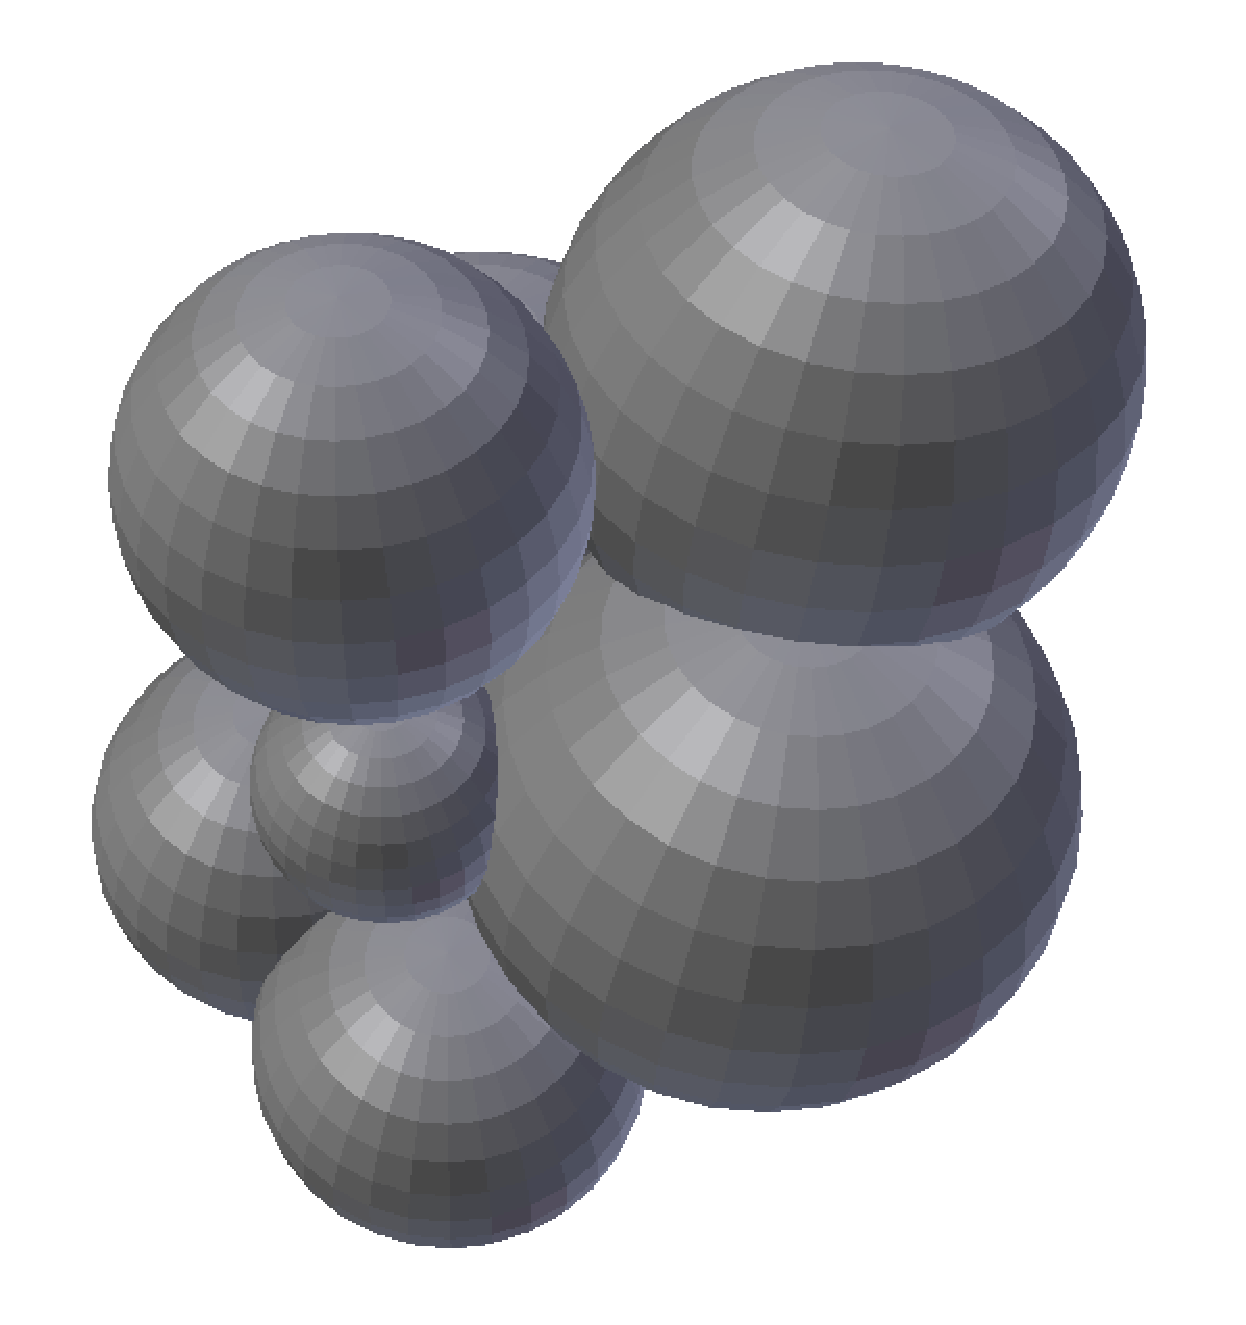
\includegraphics[width=0.45\linewidth]{figures/clunk}
		% \begin{verbatim}
		%         rand(objs)
		% \end{verbatim}
	\end{minipage}%
	\begin{minipage}[t]{5cm}
		\centering
		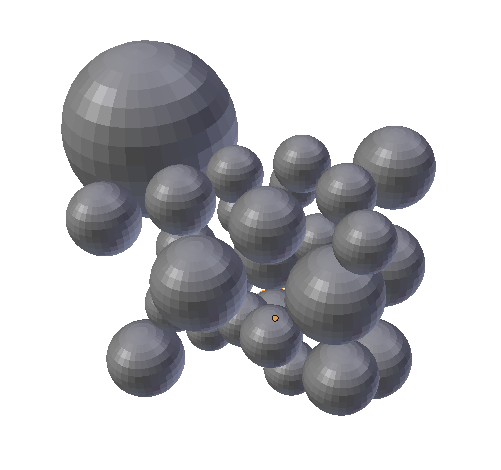
\includegraphics[width=0.45\linewidth]{figures/render}
		% \begin{verbatim}
		% pred = nointersect(objs)
		% rand(scene, pred)
		% \end{verbatim}
	\end{minipage}%
	% \begin{minipage}[t]{5cm}
	% \centering
	% 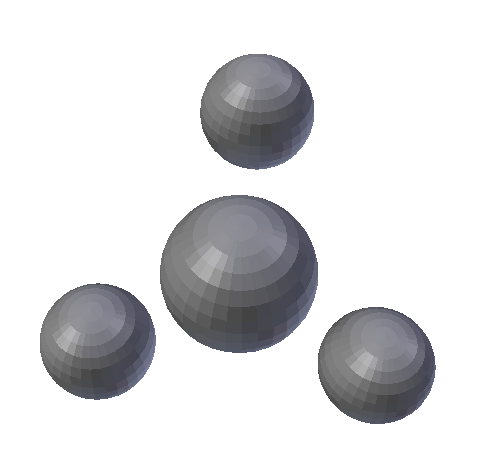
\includegraphics[width=0.5\linewidth]{figures/equi}
	% $$
	% x = 3
	% $$
	% % \begin{verbatim}
	% % pred = equidistant(objs)
	% % rand(scene, pred)
	% % \end{verbatim}
	% \end{minipage}
	\caption{A weak prior (left) does not respect rigid body constraints on objects, whereas (center) is conditioned on the predicate that objects don't intersect.  (right) objects are conditioned on being equidistant, resulting in a tetrahdral arrangement}
	\label{fig:nointersect}
\end{figure}


\paragraph{Random Variables.} Probability models lie on top of probability
spaces. A probability space is a measure space $(\Omega, {\cal H}, {\cal P})$,
where ${\cal H}$ is a sigma algebra and ${\cal P}(\Omega) = 1$ \citep{ccinlar2011probability}. Random variables are
functions from the space $\Omega$ to a realization space ${\cal X}$. As a concrete
example the space $\Omega$ can be thought of as a hypercube, with ${\cal P}$ being
uniform over that hypercube. To build a normal random variable, we need a function
that maps from $\Omega \to \mathbb{R}$. If the underlying probability space is uniform, then
this function is the inverse cumulative distribution function of the normal.

A \emph{model} $\cM$ is a collection of random variables along with a probability space.
% To fully specify a model, we need both the measure space and the
% collection of random variables on which it acts.

\paragraph{Conditioning}

Conditioning a model creates a new model.
As an example consider a model $\cM$ with two
random variables $X_1$ and $X_2$ that both take real values. Conditioning
$\cM$ on $X_1 = 1$, defines a new model $\cM_{|A}$ based on limiting the measure space
$\Omega$ to the set $A = \{ \omega : X_1(\omega) = 1\}$.
The new model is defined on a new probability space
\begin{align}
	(\Omega \cap A, \{A \cap B, B \in {\cal H} \}, {\cal P} / {\cal P}(A))
\end{align}
with the same random variables $X_1$ and $X_2$.
Sampling from $\cM_{|A}$ produces
samples only where $X_1 = 1$

More generally, conditioning on any predicate $Y(\omega) = \lk(X_1(\omega), \dots, X_n(\omega))$
defines a new model defined exactly as above, where $A = \{\omega : \lk(X_1(\omega), \dots, X_n(\omega)) = 1\}$.
% This predicate may include a comparisonsuch as $X_i < X_j$, restrict deterministic function of variables in in the model such as $\exp(X_i) = 2$, or be a Boolean combination such as $(X_i < X_j) \lor \neg(\exp(X_i) = 2)$.
Sampling from $\cM_{|A}$ generates $(x_1, ..., x_n)$ where $\lk$ is true.

The general construction of new models might require conditioning
on sets of measure zero. This process can be made rigorous
via disintegration \citep{chang1997conditioning}. Disintegration can
be thought of as the reversal of building joint distributions through
product measure constructions.


% When building models with prior beliefs via conditioning, we would like
% the property that given an infinite collection of observations, the 
% posterior predictive distribution converges to true sampling distribution.
% To study this, consider a model with two random variables that are independent,
% $X_1$ is a function of $\omega_1$ and $X_2$ is a function of $\omega_2$. Suppose
% that the true sampling distribution has $X_1$ and $X_2$ positively correlated.
% For the prior beliefs to support positive correlations, we 
% could condition on a prior belief that $X_1$ and $X_2$ are close. However
% if the form of the closeness isn't controlled by a random variable, observing
% an arbitrary amount of data from the true distribution will not change
% the dependence between $X_1$ and $X_2$ in the model. 
% \begin{align*}
% X_j^*(\omega^*) = \sigma(f_\Beta(X_{j, 1}, ..., X_{j, n})) > b, \\
% \end{align*}
% Conditioning on $X_j^*$ produces a new set of models that have 
% dependence between . Knowledge is encoded in the prior distribution
% on $\Beta$. If $f_\Beta$ has priors over the true dependence between
% $X_{., 1},...,X_{., m}$, then this new model family will converge
% to the true underlying distribution.

% rr: TODO the above can me made into a proof

% \subsection{Bayesianism vs. Bayesian Computation}
% The way we 


% \section{Higher Order Random Variables}
% People often entertain beliefs about probability statements. For instance most people accept 
% trust expert-given odds that a particular sports team will win a tournament, 
% or politician will win an election, more than the odds of those given by non-experts.
% The apparent failure of probabilistic expressions to distinguish 
% between these cases led to alternative formalisms of uncertainty \citet{Shampher}, 
% but within the probabilistic framework both \citet{Pearl} and \citet{Hyberg} demonstrated 
% that such higher order distributions were induced from the original model, no new machinery was needed.

% As a concrete example of this, suppose we have a stochastic 
% dynamical system model of human blood glucose 
% controlled by some 
% parameters $\Theta$ with a prior. A priori we know that the average blood pressure 
% in a person lives in a physically plausible range $40-400$. A way to
% encode this would be to change the prior on the parameters $p(\Theta)$ 
% to so that any sample from that prior yields has average in the physically
% plausible range. This can be challenging because it requires a detailed
% understanding of the stochastic dynamical system. 

% Alternatively, we could try to take the conditioning approach from the
% previous section. But conditioning in the previous section required explicitly
% defined random variables, and while the average glucose is a random variable
% because the parameter $\Theta$ is random, it is not an explicit random variable.
% The scenario requires the ability to both define and condition on 
% probability distributions over either random variables or properties of 
% random variables (e.g. expectations).
% In this section we introduce the random conditional 
% distribution ($\randcond$) to support this task.

% \paragraph{The Random Conditional Distribution.}
% The random conditional distribution of $X$ given $\Theta$ -- which we denote $\rcd(X, \Theta)$ or $\rcdxy{X}{\Theta}$ -- is a random distribution: a random variable which takes values in the domain of random variables.
% Informally, $\rcdxy{X}{\Theta}$ is a function of $\omega$ that returns functions of $\omega$
% of the same type as $X$. Formally, $\rcd$ is a distribution over conditional random variables:

% % The primary mechanism for conditioning is $\cond$, which constructs conditional random variables:
% % \begin{definition}
% % Let $X:\Omega \to T$ be a random variable, $Y$ an indicator function, and $\conds{X}{Y}: \Omega_{|Y} \to T$ be a conditional random variable defined as: $X_{|Y}(\omega) = X(\omega)$.
% % $X_{|Y}$ is defined on a conditioned probability space $(\Omega, \Sigma, \mu_{|Y})$ where $\mu_{|Y}$ is a conditional measure: $
% % \mu_{|Y}(A) = \mu(A \cup Y^{-1}(\{1\})) / \mu(Y^{-1}(\{1\})$.
% % % That is, $\cond: (\Omega \to T) \times (\Omega \to \{0, 1\}) \to (\Omega \to T)$ is a operator that restricts the domain of $X$ to those inputs consistent with $Y$.
% % \end{definition}


% \begin{definition}The random conditional distribution of a random variable $X: \Omega \to T_1$ given $\Theta: \Omega \to T_2$ is a random variable $\rcdxy{X}{\Theta}: \Omega \to (\Omega \to T_1)$, defined as:
% \begin{equation}\label{eq:rcd}
% (\rcdxy{X}{\Theta})(\omega) = [\conds{X}{\Theta = \Theta(\omega)}]
% \end{equation}
% \end{definition}
% For example if $\Theta = \bern(0.4)$ and $X = \normal(\Theta, 1)$, then $\rcdxy{X}{\Theta}$ is a random distribution 
% whose domain comprises of two normal distributions $X_1 = \conds{\normal(\Theta, 1)}{\Theta = 1}$ and $X_2$.
% The probabilities of $X_1$ and $X_2$ with respect $\rcdxy{X}{\Theta}$ are determined by the prior probabilities of the different outcomes of $\Theta$: $P((\rcdxy{X}{\Theta}) = X_1) = 0.4$ and $P((\rcdxy{X}{\Theta}) = X_2) = 0.6$.

% A random conditional distribution is most useful in combination with other functions.
% Expectation is perhaps the most important example, which when composed with $\rcd$ produces conditional expectation.
% Restricting to real valued variables, expectation $E$ is a functional that maps a random variable to a real value
% (($\Omega \to \mathbb{R}) \to \mathbb{R}$).
% When $X$ is a real valued random variable, $\rcdxy{X}{\Theta}$ is not real valued, and hence not a valid argument to $E$.

% However, just as arithmetic operations such as $+$ and $-$ extend from the domain of numbers to the domain of random variable (pointwise $X + Y = \omega \mapsto X(\omega) + Y(\omega)$), $E$ extends from the domain of random variables to the domain of random variables over random variables in precisely the same way.
% % Since random variables are themselves functions, $E$ is an operator, functional or more generally a higher-order function.  
% % As described in section X a function with domain $T$ can be lifted to a functional of $T$-valued random variables.
% % $T$ is purposefully left abstract, because in addition to lifting functions defined on the reals etc, we can lift functions defined on random variables.
% % Expectation is a cannonical example of a random variable valued function, with type $E : (\Omega \to \mathbb{R}) \to \mathbb{R}$.
% That is, $\ee$ has a lifted counterpart $\lifted{\ee} = \lift(\ee)$ with type $\lifted{\ee} : (\Omega \to (\Omega \to \mathbb{R})) \to (\Omega \to \mathbb{R})$, which maps a distribution over real valued random variables to a distribution over real values (expectations).
% % $$
% % \lifted{\ee}(X)(\omega) = \mean{X(\omega)}
% % $$
% The operator $\rcd$ composed with $\ee$ constructs conditional expectation (with respect to a random variable $\Theta$):
% \begin{equation}
% \lmean{\rcdxy{X}{\Theta}} = \lmean{\omega \mapsto \conds{X}{\Theta = \Theta(\omega)}} 
%                     = \omega \mapsto \mean{\conds{X}{\Theta = \Theta(\omega)}}\\
% \end{equation}
% The final term $\omega \mapsto \mean{\conds{X}{\Theta = \Theta(\omega)}}$ matches the definition of
% conditional expectation
% with respect to a random variable $\mean{(X\mid \sigma (Y))(\omega)} = \mean{X \mid Y = Y(\omega))}$.
% That is the conditional expectation is a random variable with randomness provided by the conditioning set.

% Returning to the blood glucose example, we can build a model that respects the valid range
% of average blood glucose by taking the original model creating the conditional expected
% value of glucose $G$ with $\rcd$ and expectation of $\rcd$, then constructing a new model
% by conditioning the original on $G$ being in the physiologically possible range.

% \paragraph{Completeness.}Nested uses of $\rcd$ lead to a completeness result. State informally: 
% by repeatedly applying $\rcd$, any random function or functional in the original model
% can be constructed. Then by using conditioning to create new models from the previous 
% section, we can alter existing models to respect predicates on any random quantity in
% the model even if the random quantity is not an explicit random variable.
% % RR: TODO: The above could be a theorem


%% \section{Higher Order Probabilistic Inference}

% People often entertain beliefs about probability statements.
% For instance most people accept even expert-given odds that a particular sports team will win a tournament, or politician will win an election, with a degree of scepticism.
% % and therefore (iii) perhaps we need a new or extended theory of probability to be able to reason about these facts.
% The apparent failure of probabilistic expressions to distinguish between these cases led to alternative formalisms of uncertainty \cite{Shampher}, but within the probabilistic framework both Pearl \cite{} and HyBerg{} demonstrated that such higher order distributions were induced from the original model, no new machinery was needed.
% Many scenarios require the ability to both define and condition probability distributions over either random variables or properties of random variables (e.g. expectations).
% In this section we introduce the random conditional distribution ($\randcond$) to support this task.
% $\rcd$ is best explained through example:


% % Higher order probabilities emerge whenever there is a distinction between subjective and objective probabilities.
% % For example many systems which verify probabilistic statements make assertions such as this assertion holds with a probability greater than 0.9.
% % This distinction between the objective probability with which the assertion holds and the bound that can be proved reflects the gap in the reasoning capacity of the agent.

% % Further still, higher order distributions is a more general concept that higher order probabilities, encompassing it as a special case.
% % Consider an assertion about the fairness of a hiring program $P$ that takes as input a vector of arguments $v$ representing a job applicant’s record and returns a Boolean value indicating whether the applicant is hired.
% % One of the arguments $v$ 


% Consider a coin toss in the basement of a unscrupulous gambler, and having the belief that the coin could be fair or be biased towards tails, but also that the coin-tosser may bias its outcome through sleight of hand.

% \begin{figure}[!htb]
% \centering
% 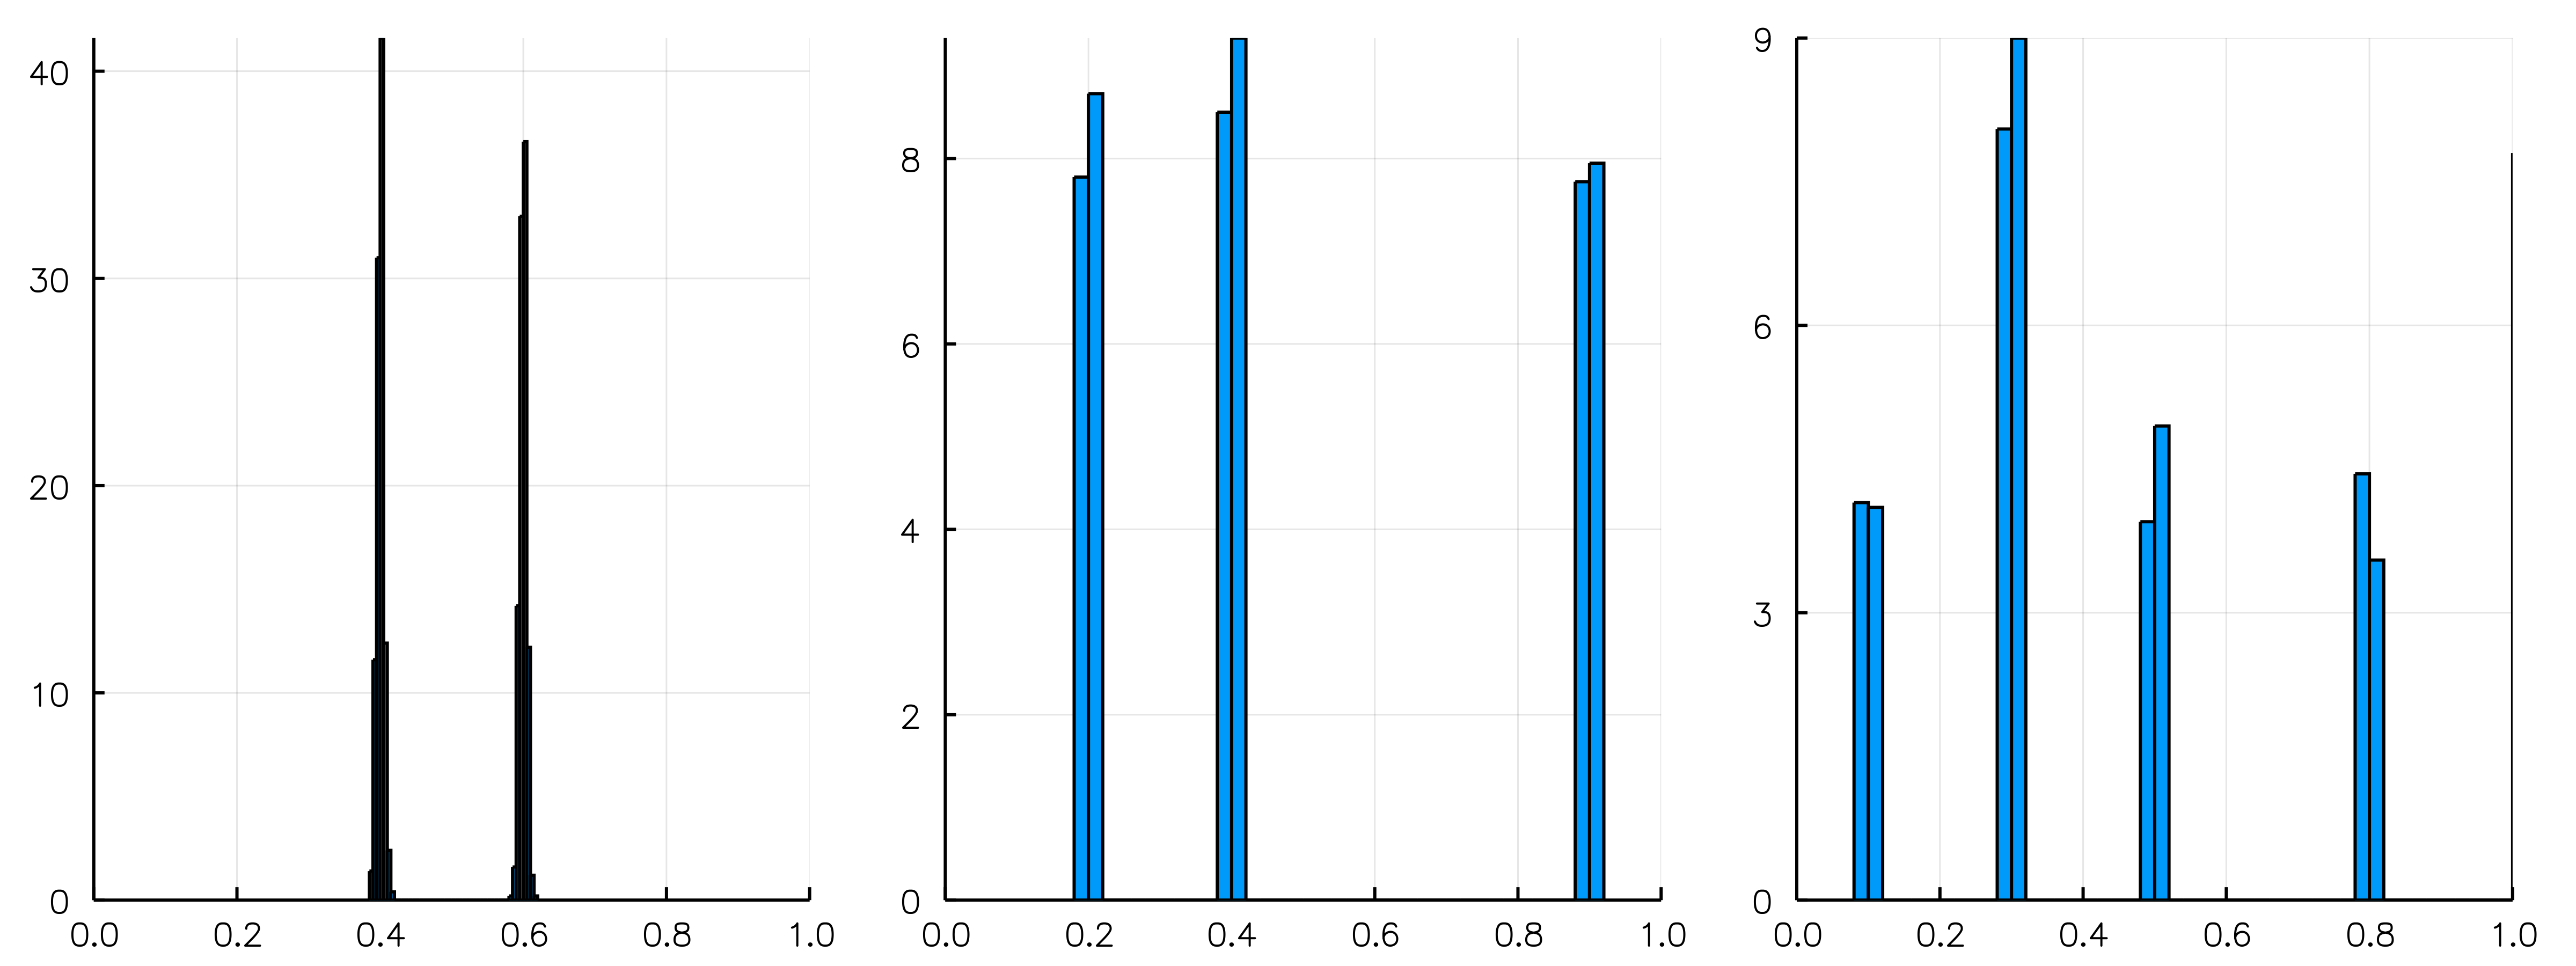
\includegraphics[width=0.9\linewidth]{figures/rcd}
% \caption{Imagine observing the outcome of flips of a coin of unknown fairness, e.g., $coin = \bern(w + b)$ comes up heads with probability $W + b$, where weight $w = \unif(\{-0.2, 0, 0.2\})$ is uniformly distributed,  $b = \unif(\{-0.2, 0, 0.5\})$
% The marginal probability that the $P(coin = H) = 0.5$ is equal to that of a bank-minted, fairly-tossed coin.
% Put another way, despite the fact that a gamblers coin tossed by untrustworthy tosser and a freshly minted coin have the same overall probability of turning up heads, we would not be very surprised if the fraction of heads appearing in a large number of the gambler coin tosses deviated greatly from 0.5, but very surprised if it occurred with bank coin tosses.
% The random conditional distribution allows us -- among other things -- to induce distributions over probabilities directly from the original model, distinguishing these two scenarios.
% \ref{rcd} demonstrates .  From left to right random samples from (a) $\mean{\rcd(coin, fair)}$, (b) $\mean{\rcd(coin, b)}$ (c) $\mean{\rcd(coin)}$}
% \label{fig:rcd}
% \end{figure}

% TODO: Higher order more general that reasoning over beliefs





% \subsection*{Lifting}
% Lifting is a process which gives meaning to expressions such as $X+X$ when $X$ is a random variable rather than a number.
% To lift a function (such as $+$) means to It constructs a functional defined on $T$-valued random variables from a function defined on values of type $T$, mechanising the principle that a transformation of a random variable yields a random variable.
% Lifting is important because syntactically, it is more convenient to use random variables as if they were values rather than compose functions in measure theoretic notation.
% In addition, it allows us to repurpose existing programs expressed in values of type $T$ (e.g., ray-tracers which take geometric objects as input) to $T$-valued random variables (distributions over objects), without modification.

% To treat random variables as values we interpret operations on them \emph{pointwise}.
% % Given a function $f$ with domain $T$, we lift it to the domain of a random variable of codomain $T$.
% Let $X:\Omega \to T_1$ be a random variable, and $f:T_1 \to T_2$ be a function, then $Y = f(X)$ is a random variable defined as:
% $$
% Y(\omega) = f(X(\omega))
% $$
% Lifting extends to multivariate functions in the obvious way, e.g.:
% $$
% X + X = \omega \mapsto X(\omega) + X(\omega)
% $$
% More generally lifting is performed through an operator $\lift$:
% \begin{definition}
% Let $f: T_i \times \cdots \times T_n$ be an $n$-ary multivariate function, and denote by $e_\omega()$ the evaluation functional defined by $e(X, \omega) = x(\omega)$ if $X$ is a random variable and $e(X, \omega) = X$ otherwise.
% $\lifted{f}: (\omega \to T_1) \times \cdots \times (\omega \to T_n)$ where $f(X)$
% \end{definition}

% \improvement{WHY is lifting defined pointwise}

% \subsection*{Conditional Random Variable}
% Probabilistic inference is achieved through conditioning.
% To condition means to restrict the universe to only those scenarios where a condition holds.
% A predicate $Y: \Omega \to \{0,1\}$ can be used to restrict a probabilistic model to a subset of the uncertainty.
% That is, every event $A$ has a characteristic predicate $Y$ defined by
% $Y(\omega) = 1$ if $\omega \in A$, otherwise $Y(\omega) = 0$.
% Equivalently, the image of $A$ under $Y$ is $\{1\}$ and the preimage of $\{1\}$ under $Y$ is $A$ is 
% $Y^{-1}(\{1\}) = \{ \omega \in \Omega : Y(\omega)\} = A$

% The primary mechanism for conditioning is $\cond$, which constructs conditional random variables:
% \begin{definition}
% Let $X:\Omega \to T$ be a random variable, $Y$ an indicator function, and $X_{|Y}: \Omega_{|Y} \to T$ defined as $\cond(X, Y)$ be a conditional random variable defined as: $X_{|Y}(\omega) = X(\omega)$.
% $X_{|Y}$ is defined on a conditioned probability space $(\Omega, \Sigma, \mu_{|Y})$ where $\mu_{|Y}$ is a conditional measure: $
% \mu_{|Y}(A) = \mu(A \cup Y^{-1}(\{1\})) / \mu(Y^{-1}(\{1\})$.
% That is, $\cond: (\Omega \to T) \times (\Omega \to \{0, 1\}) \to (\Omega \to T)$ is a operator that restricts the domain of $X$ to those inputs consistent with $Y$.
% \end{definition}

% Conditional random variables.  Operations on conditional random variables constructs further conditional random variables.
% Observe that if two conditional random variables are composed then:

% $$
% \begin{aligned}
% (f(X_{|Y}))(\omega)&=f(X_{|Y}(\omega))&{\text{ where } Y(\omega)}\\
% (f(X_{|Y_1}, X_{|Y_2}))(\omega)&=f(X_{|Y}(\omega))&{\text{ where } Y_1(\omega)} \wedge Y_2(\omega)\\
% % (\lambda f)(x)&=\lambda \cdot f(x)&{\text{(pointwise multiplication by a scalar)}}
% \end{aligned}
% $$

\section{The Random Conditional Distribution}
The random conditional distribution of $X$ given $\Theta$ -- which we denote $\rcd(X, \Theta)$ or $\rcdxy{X}{\Theta}$ -- is a random distribution: a random variable which takes values in the domain of random variables.
Informally, $\rcdxy{X}{\Theta}$ is a probability distribution over random variables of the same type as $X$, where each random variable in that distribution corresponds to an element of $\theta \in \Theta$ and is weighted by the prior probability of $\theta$.
Formally, $\rcd$ is a distribution over conditional random variables:

% The primary mechanism for conditioning is $\cond$, which constructs conditional random variables:
\begin{definition}
Let $X:\Omega \to T$ be a random variable, $Y$ an indicator function, and $\conds{X}{Y}: \Omega_{|Y} \to T$ be a conditional random variable defined as: $X_{|Y}(\omega) = X(\omega)$.
$X_{|Y}$ is defined on a conditioned probability space $(\Omega, \Sigma, \mu_{|Y})$ where $\mu_{|Y}$ is a conditional measure: $
\mu_{|Y}(A) = \mu(A \cup Y^{-1}(\{1\})) / \mu(Y^{-1}(\{1\})$.
% That is, $\cond: (\Omega \to T) \times (\Omega \to \{0, 1\}) \to (\Omega \to T)$ is a operator that restricts the domain of $X$ to those inputs consistent with $Y$.
\end{definition}


\begin{definition}The random conditional distribution of a random variable $X: \Omega \to T_1$ given $\Theta: \Omega \to T_2$ is a random variable $\rcdxy{X}{\Theta}: \Omega \to (\Omega \to T_1)$, defined as:
\begin{equation}\label{eq:rcd}
(\rcdxy{X}{\Theta})(\omega) = \conds{X}{\Theta = \Theta(\omega)}
\end{equation}
\end{definition}
For example if $\Theta = \bern(0.4)$ and $X = \normal(\Theta, 1)$, then $\rcdxy{X}{\Theta}$ is a random distribution comprised of two normal distributions $X_1 = \conds{\normal(\Theta, 1)}{\Theta = 1}$ and $X_2$.
The probabilities of $X_1$ and $X_2$ with respect $\rcdxy{X}{\Theta}$ are determined by the prior probabilities of the different outcomes of $\Theta$: $P((\rcdxy{X}{\Theta}) = X_1) = 0.4$ and $P((\rcdxy{X}{\Theta}) = X_2) = 0.6$.

A random conditional distribution is most useful when used in combination with other functions.
Expectation is perhaps the most important example, which when composed with $\rcd$ produces conditional expectation.
Expectation $E : (\Omega \to \mathbb{R}) \to \mathbb{R}$ is a functional that maps a random variable to a real value.
When $X$ is a real valued random variable, $\rcdxy{X}{\Theta}$ is not real valued, and hence not a valid argument to $E$.
However, just as arithmetic operations such as $+$ and $-$ extend from the domain of numbers to the domain of random variable (pointwise	 $X + Y = \omega \mapsto X(\omega) + Y(\omega)$), $E$ extends from the domain of random variables to the domain of random variables over random variables in precisely the same way.
% Since random variables are themselves functions, $E$ is an operator, functional or more generally a higher-order function.  
% As described in section X a function with domain $T$ can be lifted to a functional of $T$-valued random variables.
% $T$ is purposefully left abstract, because in addition to lifting functions defined on the reals etc, we can lift functions defined on random variables.
% Expectation is a cannonical example of a random variable valued function, with type $E : (\Omega \to \mathbb{R}) \to \mathbb{R}$.
That is, $\ee$ has a lifted counterpart $\lifted{\ee} = \lift(\ee)$ with type $\lifted{\ee} : (\Omega \to (\Omega \to \mathbb{R})) \to (\Omega \to \mathbb{R})$, which maps a distribution over real valued random variables to a distribution over real values (expectations).
$$
\lifted{\ee}(X)(\omega) = \mean{X(\omega)}
$$
$\rcd$ composed with $\ee$ constructs conditional expectation (with respect to a random variable $\Theta$):
\begin{equation}
\lmean{\rcdxy{X}{\Theta}} = \lmean{\omega \mapsto \conds{X}{\Theta = \Theta(\omega)}} 
                    = \omega \mapsto \mean{\conds{X}{\Theta = \Theta(\omega)}}\\
\end{equation}
The final term $\omega \mapsto \mean{\conds{X}{\Theta = \Theta(\omega)}}$ is the definition of a conditional expectation with respect to a random variable $\mean{(X\mid \sigma (Y))(\omega)} = \mean{X \mid Y = Y(\omega))}$.

% Move to appendix?
% Equation \ref{eq:rcd} is a construcive definition of $\rcd$; here we define it declaratively:
% Let $\mu_\Theta = \mu \circ \Theta^{-1}$ denote the push forward measure of		 $\mu$ with respect to $\Theta$, $\tilde{X} = \randcond(X, \Theta)$, and $X^* \subset \tilde{X}$ be a set of random variables, then:
% $$
% \mu_{\tilde{X}}(X^*) = \mu_\Theta(\varphi^{-1}(X^*))
% $$

\improvement{This needs to be made clearer. Will there be issues taking measures in function space?}

\improvement{Need to define space of functions that measures exist on. Then define curry(X, $\Theta$), random variable on functions, to take measure given by pullback to $\Theta$ }

\improvement{Define: RCD of one argument $\rcd(X)$}

% \subsection{Higher Order Graphical Model}

% Probabilistic inference means to construct and condition random variables.
% In measure theory, a random variable is a function from a sample space $\Omega$ to $T$, where $T$ could for example be $\mathbb{R}$, but any type in general.
% $\Omega$ is understood as the universe of possible scenarios that could occur, or in sampling terms, as the random inputs to a random variable.
% Measure theory formalizes uncertainty by assigning probabilities to sets of possible scenarios, called events.
% The measure of an event represents a degree of belief that the event could occur, and is determined by a probability measure $\mu:\Sigma \rightarrow [0,1]$ where $\Sigma$ is a sigma-algebra (measurable subsets of $\Omega$).
% An event $A$ is impossible if $\mu(A)=0$, and certain if $\mu(A)=1$.

% We formulate $\rcd$ with respect to a form of directed graphical model.
% Higher order directed graphics are similar to standard bayesian networks but depart from them in two significant ways.
% First, the semantics of a graph is defined in terms of measure theoretic random variables, in contrast to probability mass or density functions, which means that every node is a deterministic transformation and all randomness is considered external to the system.
% Second this graph formalism is based on measure theoretic probability.

% \begin{definition}
% A higher order Bayesian Network $\mathcal{G}(V,E)$ is a directed acyclic graph, where $V$ are the nodes and $E$ are the edges of the graph.
% Nodes correspond to random variables, measurable functions from a sample space $\Omega$ to some output type $T$.
% Let $V_{\omega} \subseteq V$ denote the subset of variables without parents.
% Higher order graph are able to express both functions between  variables and functions of variables.
% Standard (non higher order) models are expressed using edges in $E_\circ$ (read $E$ compose).
% A composition edge from $A$ to $B$ denotes that $B$ functionally (and causally) depends on $A$.
% More precisely $A \to B$ denotes the composition $B \circ A$.
% Since $A$ is random variable, this composition is a random variable $\omega \mapsto B(A(\omega))$.
% \end{definition}
% Application edges in $E_{apply}$ denote function application.
% If a node $A$ is at the source of a directed edge in $E_{apply}$ it is taken as a value to be given as input to the node at the tail.
% % Let $f : V \to what$ map each node to a corresponding function, and $id : V_{\omega} \to \mathbb{N}$ map each parent-free node to a unique integer.
  
% \begin{align*}
% \mu &= \mathcal{N}(0, 1) \\
% X &= \mathcal{N}(\mu, 1) \\
% \tilde{X} &= \mathbb{E}(\rcdxy{X}{Y})
% \end{align*}


% \subsection{Efficient Construction of the Random Conditional Distributions}

Each outcome of a random conditional distribution is a conditional random variable which, in the general setting, can be a challenge to sample from.
In this section we demonstrate how to efficiently construct the random conditional distribution in a wide class of scenarios.

Recall that $(\rcdxy{X}{\Theta})(\omega) = \conds{X}{\Theta = \Theta(\omega)}$.
A realization $\conds{X}{\Theta = \Theta_c}$ of $\rcdxy{X}{\Theta}$ is a conditional random variable which may be difficult to sample from.
Instead, under modest conditions (theorem \ref{thm:path}) it is permissible to use a different distribution which is easier to construct:  $\ridxy{X}{\Theta}$ which \emph{fixes} rather than conditions $\Theta$:
\begin{equation}\label{eq:rid}
(\ridxy{X}{\Theta})(\omega) = \conds{X}{\Theta^a = \Theta^a(\omega) \text{ for all } \Theta^a \in \{ \Theta \} \cup \text{ancestors of } \Theta}
\end{equation} 
$\rcdxy{X}{\Theta}$ is distinct from $\ridxy{X}{\Theta}$ because in the former the parents of $\Theta$ are not fixed and hence for some realization $\conds{X}{\Theta = \Theta_c}$ we must consider all the possible scenarios which would result in $\Theta = \Theta_c$.
In contrast, 
$\ridxy{X}{\Theta}$ is always efficient to construct:

\begin{algorithm} 
\end{algorithm}

It is permissible to use $\ridxy{X}{\Theta}$ as a substitute for $\rcdxy{X}{\Theta}$ when they are equivalent, which is not always the case, consider:
\begin{align*}
\alpha &= \rade(0.5) \\
\beta &= \bern(0.5) * \alpha \\
\gamma &= \bern(0.5) + \alpha + \beta
\end{align*}

Random conditional distributions (such as $\rcdxy{\gamma}{\beta}$) can be induced from this model which are not equal to the corresponding "fixed" random conditional distribution: $\ridxy{\gamma}{\beta}$.
For example the distribution over expectations $\lmean{\rcdxy{\gamma}{\beta}}$ and $\lmean{\ridxy{\gamma}{\beta}}$ do not even have the same support.
However in other scenarions they are the same, e.g. $\rcdxy{\gamma}{\alpha} = \ridxy{\gamma}{\alpha}$.

Verifying equivalence of two random variables (let alone two random distributions) is undecidable in theory \ref{} and intractable in practice, putting us at risk of swapping one hard problem for a harder one.
Fortunately, the causal structure of the model provides sufficient (but not neccesary)ee conditions to determine if $\ridxy{X}{\Theta} = \rcdxy{X}{\Theta}$:
% Intuitively, the first result can be substitued because it sucks, while the seon dosn't suck.

\todo{Maybe use d-separation. $\Theta$ d-separates $X$ from its ancestors}
\begin{theorem} $\rcdxy{X}{\Theta} = \ridxy{X}{\Theta}$ when all paths from the ancestors $\Theta$ to $X$ pass through $\Theta$
\end{theorem}
\begin{proof}
To prove this theorem, it is crucial to formalize the structural assumption. The ancestors of $\Theta$ have no path to $X$ that doesn't pass through $\Theta$. This means that conditioned on $\Theta$, any ancestor of $\Theta$, $\Theta^a$, is independent from $X$, i.e.
\begin{equation*}
\conds{X}{\Theta, \Theta^a} = \conds{X}{\Theta} \quad \text{for all } \Theta^a \in \text{ancestors of } \Theta
\end{equation*}
Therefore, using \eqref{eq:rid} we obtain the following identity for all $\omega$
\begin{equation*}
(\ridxy{X}{\Theta})(\omega) = (\conds{X}{\Theta = \Theta(\omega), \Theta^a = \Theta^a(\omega) \text{ for all } \Theta^a \in \text{ancestors of } \Theta}) = \conds{X}{\Theta = \Theta(\omega)}
\end{equation*}
which concludes the proof that $\rcdxy{X}{\Theta} = \ridxy{X}{\Theta}$.
\end{proof}

% For example, to construct a set of samples from $\mean{\rcdxy{X}{Y}}$, we could:
% \begin{itemize}
% \item Unconditionally sample $Y$ to yield $y_c$.
% \item Sample $X^*$ from $\tilde{X}$ such that $X^* = X \mid Y = y_c$, where $y_c = Y(\omega_c)$ is a realization of $Y$
% \item Find $\Omega^* \subset \Omega$ such that $Y(\omega^* \in \Omega^*) = y$
% \item Compute $\mean{X^*}$ with respect to $\Omega^*$
% \end{itemize}

% Step 2 is hard for all the same reasons that conditioning is hard in general.
% However, we can exploit the fact that the condition $Y = Y(\omega)$ in $\rcdxy{X}{Y}$ is not an arbitrary condition, in effect, it is conditioning on the prior.

% \begin{itemize}
%   \item Unconditionally sample $Y$ to yield $y_c$, cache its input $\omega_c$ (i.e., $Y(\omega_c) = y_c$)
%   \item Compute $\mean{X}$ 
% \end{itemize}

% This sequence is identical in distribution to the first sequence, but dramatically easier to compute.

\section{Omega}
Omega is a probabilistic programming system based on the measure theoretic probability theory described in Section \ref{condknow}.
As a system, Omega is implemented in the Julia programming language \citep{bezanson2017julia}, but the principles upon which it is built can be supplanted into many existing programming languages.
Omega is designed so that the sample space $\Omega$ is a first-class object referred to explicitly in probabilistic models, and manipulated to perform inference. 
This contrasts the general setup in
measure theoretic probability where the structure
of $\Omega$ is only made explicit when proving the
existence of certain types of random structures.

The approach we take defines models by the probability 
space $(\Omega, {\cal H}, {\cal P})$ and a collection
of functions on it to provide random variables. 
This approach requires an explicit construction for the
the structure of $\Omega$ to support all kinds
of random variables we wish to express, including both continuous and discrete, bounded and unbounded.
We represent $\Omega$ as a $d$-dimensional unit hypercube $[0, 1]^d$ where $d$ may be finite or infinite and is determined implicitly by the random variables defined on it.

In our approach, random variables are pure functions of $\Omega$ and provide 
the sole mechanism for constructing probabilistic models.
This contrasts probabilistic programming languages such as Stan~\citep{carpenter2017stan}, Church~\citep{goodman2008church}, Venture~\citep{mansinghka2014venture} and Anglican~\citep{wood2014new} which take stochastic simulators as the principal mechanism for defining probabilistic models.
Although there are clear connections between a random variable and a stochastic simulator---a sampler is a random variable paired with source of randomness---there are important differences.
To define a random variable, we define a function, which transforms an element $\omega \in \Omega$. For example to define a variable \texttt{x} with a particular distribution, we 
can apply its inverse cumulative distribution function to its input parameter \texttt{omega}$\in \Omega$.
\begin{figure}[h]
\centering
\begin{BVerbatim}
x(omega) = invcdf(omega)
\end{BVerbatim}
\end{figure}\\\textbf{}
One quirk of the measure theoretic approach is that random variables, unlike samplers, are not automatically (conditionally) independent. This is because all random variables are functions of the entire probability space.
To facilitate the construction of independent random variables,  
Omega includes a function $\iid$.
$\iid(x)$ is a copy of $x$ that it is conditionally independent (given dependents) and identically distributed:
\begin{figure}[h]
	\centering
	\begin{BVerbatim}
x1 = iid(x); x2 = iid(x); ...
	\end{BVerbatim}
\end{figure}\\
It works by having each copy of $x$ be a function of a different dimension
of $\omega$. More complex random variables are made by either defining more complex functions or by composing random variables as if they were values.

Operations on random variables are defined pointwise.  The following two definitions, \texttt{y1} and \texttt{y2}, are identical:
\begin{figure}[h]
	\centering
	\begin{BVerbatim}
y1 = x + x; y2(omega) = x(omega) + x(omega)
\end{BVerbatim}
\end{figure}\\
% Pointwise operations on random variables is the prime mechanism in which they are made dependent.  For example if \texttt{x} is a random variable then $y = ciid(normal(x, y))$ has \textrm{x} as a parent composition, and unrolled would be defined as
% y(omega) = normal() + x(omega) * 1
We assume the existence of an external source of randomness that allows us through a procedure $\rand$ to construct an element in $\Omega$ according to its measure.
\begin{center}
\begin{minipage}{5cm}
\begin{Verbatim}[fontsize=\small]
omega = rand(Omega)
\end{Verbatim}
\end{minipage}
\end{center}
Random variables can be applied as functions to elements in $\Omega$. For instance:
\begin{center}
\begin{minipage}{5cm}
\begin{Verbatim}[fontsize=\small]
w = rand(Omega); x(w)
\end{Verbatim}
\end{minipage}
\end{center}
draws a sample from the distribution of $X$. Direct samples of a random variable can be sampled with \texttt{rand(X) = X(rand(Omega))}. 

The last operation Omega defines is conditioning. Conditioning builds new random variables by restricting the value of another. This can be used:
\begin{center}
\begin{minipage}{5cm}
\begin{Verbatim}[fontsize=\small]
x = cond(x, y)
\end{Verbatim}
\end{minipage}
\end{center}
The result is that a model in Omega resembles the underlying mathematical model. Take the process of drawing from a normal with random mean, then conditioning on that
random mean take value $1$. This can be expressed in Omega as
\begin{center}
\begin{minipage}{5cm}
\begin{Verbatim}[fontsize=\small]
mu = iid(normal(0, 1))
x  = iid(normal(mu, 5))
cond_x = cond(x, mu == 1)
rand(cond_x)
\end{Verbatim}
\end{minipage}
\end{center}
% zenna: the above needs a more compelling example
It is important to emphasize that while the code does not look that different from code one could write in languages like Church, the semantics are quite different in that the first two lines are not sampling from a normal distribution: they are defining \texttt{mu} and \texttt{x} as random variables. The program is then deriving a new random variable \texttt{cond\_x} by conditioning on them; sampling only happens explicitly in the last line. In general, with the primitives defined above, 
Omega allows for the construction of general random variables,
conditional random variables, and simulation from these random variables. 

\subsection{Inference}
In general it is easy to construct a transformation of a random variable 
and simulate from it, but intractable to compute the corresponding transformed mass or density function. 
% In Omega one can define and condition on arbitrary transformations of random variables with intractable  likelihood and as a result, more often than not we will be in the regime where computation of the likelihood is intractable and hence we develop a likelihood-free inference method
To support conditioning on arbitrary transformations of random variables we develop a method of inference that avoids computing the likelihood all together.
In particular, the inferential task we address is to sample from the conditional distribution $\conds{X}{Y}$, constructed with \texttt{cond(x,y)} in Omega.
We:
\begin{enumerate}
	\item Reframe the problem. Rather than sample from the random variable $\conds{X}{Y}$ directly, we aim to first sample from the \emph{conditional set} $C(Y) = \{ \omega \in \Omega \mid Y(\omega) = 1 \}$. 
With a conditional sample in $\Omega$, a conditional sample from $X$ is straightforward to compute by forward execution of the function defining $X$, i.e. $X(\omega)$.
\item Sampling $\omega \in C(Y)$ is often intractable, as it can require the inversion of a complex, nonlinear function.
We instead approximate $Y$ with an unnormalized density function $U_Y: \Omega \to [0, 1]$, which is constructed to be consistent with $Y$ on values of $\omega \in C(Y)$, but smoothly degrade to zero on $\omega$ outside the conditioning set,  
\item Perform inference on $U_Y$.  The softening of the constraint on $\Omega$ to a density allows us to apply inference algorithms.  In particular, we construct a Markov Chain exploring $\Omega$ whose stationary distribution is $U_Y$.  Intuitively, this is constructing a random walk through the random inputs of a probabilistic program to find those which satisfy specified conditions. At the end of this section we will describe how other inference techniques can be used as well.
\end{enumerate}

There are three desiderata which govern how the unnormalized density -- or simply energy -- function  $U_Y$ approximates $Y$.  First, we would like $U_Y$ to have a temperature parameter $\alpha$ that controls the fidelity
of the approximation. In particular, we want $U_Y$ to converge to $Y$ as $\alpha \to 0$, and to converge to a flat surface as $\alpha \to \infty$. Second, temperature should vary monotonically with the fidelity of the approximation, parameterizing a tradeoff between accuracy of samples and ease of inference. Third, we want to preserve consistency with $Y$. That is $Y(\omega) = U_Y(\omega)$ when $\omega \in C(Y)$, at all temperatures.  This consistency is one-sided; we do not, and could not, require it also hold at 0 and preserve the other desiderata.

% The family of approximations of the predicate $Y$ is parameterized through a temperature $\alpha$ that controls the smoothness of the approximation. In particular, $U_Y$ with $\alpha \to 0$ converges to $Y$ itself while increasing values of $\alpha$ yield smoother approximations eventually giving a flat surface when $\alpha \to \infty$. Moreover, the set of conditional samples $C(Y) = \{ \omega \in \Omega \text{ } | \text{ } Y(\omega) = 1 \}$ are assigned a value of $1$ in $U_Y$ for all temperatures. 

In most scenarios $U_Y$ is induced by defining a distance function on random variables in the model. 
For example if $X_1$ and $X_2$ are real valued random variables, then replace the predicate $X_1 = X_2$ with the energy function $U_Y = e^{-\rho(X_1, X_2) / \alpha}$ where $\rho$ is a distance function on the outcome space of $X_1$ and $X_2$.
This satisfies the desiderata outlined above.  We then call $U_Y$ a permissible approximation $Y$
% To construct a $U_Y$ with such properties, we let $Y$ be the following predicate $a=b$ for standard Gaussians $a, b \sim \mathcal{N}(0, 1)$. We choose a distance
% $\rho(a, b)$ to indicate how close our sample is to $C(Y)$. To meet the desiderata
% of having $C(Y)$ be $1$ over the constraint set and to ensure the constraint becomes
% smoother with large $\alpha$, we use a function $k : [0, \infty] \to [0, 1]$ parameterized by $\alpha$ to wrap the distance $\rho(a, b)$. A simple choice for such a function is $k(d; \alpha) = e^{-d / \alpha}$ that provides the desired properties to $U_Y$ (see Appendix). The formal definition of $U_Y$ is as follows.

\begin{definition}
The function $U_Y : \Omega \to [0, 1]$ parameterized by $\alpha$ is an approximation of a predicate $Y$ if:
\begin{enumerate}[label=(\roman*)]
	\label{def:temp}
	\item For all $\omega \in \Omega$, the limits $\lim_{\alpha \to 0}U_Y(\omega; \alpha) = Y(\omega)$ and $\lim_{\alpha \to \infty}U_Y(\omega; \alpha) = 1$ hold.
    \item For all $\alpha \in [0, \infty)$ and  $\omega \in C(Y)$, $U_Y(\omega; \alpha) = 1$.
    \item The increasing fidelity is characterized by entropy, i.e. the entropy $H(U_Y(\omega; \alpha))$ of the unnormalized density $U_Y$ is an increasing function of $\alpha$.\footnote
    {By compactness, it is integrable for all $\alpha$, when $\Omega$ has finite dimension}
\end{enumerate}
\end{definition}

We derive $U_Y$ from $Y$ semi-automatically. 
Recall that a probabilistic model $\mathcal{M}$ is a collection of random variables on a shared probability space, and that a predicate $Y \in \mathcal{M}$ is generally a composition of these variables.
We derive $U_Y$ from $Y$ by replacing all predicates (Boolean valued functions) in $Y$ with corresponding relaxations defined on $\mathbb{R}$.
In programming language terminology this is a nonstandard execution of $Y$ and can be implemented by a source to source transformation of the code which comprises $Y$.
In Omega we achieve the same result through use of the multi-method dispatch, which is similar to operator overloading by allowing multiple methods to use the same name if distinguished by type.  That is, we define a distinct type for primitive types (such as $\mathbb{R}$), and redefine Boolean operators on these types to their softened counterparts.

Probabilistic models are compositions of a small number of primitive operations, hence the burden of constructing softened predicates need only be done once.
Generally our soft predicates $\tilde{z} = \soft(z)$ take the form $k(\rho(a, b); \alpha)$.
Here the function $\rho(\cdot, \cdot)$ is a distance metric between two points (or with abuse of notation set of points).
% On the other hand, $k : [0, \infty] \to [0, 1]$ parameterized by the temperature $\alpha$ maps a distance to the relaxation of the predicate such that $d = 0 \Longleftrightarrow k(d; \alpha) = 1$.

\begin{center}
\begin{tabular}{ l | c | c | c | c |r }
  \hline		
  $z$ & $a = b$ & $a > b$ & $a < b$ & $a \land b$ & $a \lor b$  \\
  $\tilde{z}$ & $k(\rho(a, b))$ & $k(\rho(a, [b, \infty]))$ & $k(\rho(a, [-\infty, b]))$ & $\min(\tilde{a}, \tilde{b})$ & $\max(\tilde{a}, \tilde{b})$\\
  \hline  
\end{tabular}
\end{center}


% The formal choice for $k(\cdot ; \cdot)$ that satisfies the conditions in Definition \ref{def:temp} is given by $k(d; \alpha) = \mathbbm{1}_{d=0} e^{-d \alpha} + \mathbbm{1}_{d \neq 0} e^{-d / \alpha}$ (see Appendix). 
% Practically, we never encounter $\alpha = 0$ so we replace the aforementioned function with the equivalent and simpler $k(d; \alpha) = e^{-d / \alpha}$. 
% Adjusting the value of the temperature $\alpha$ from $\infty$ to $0$ illustrates the fundamental tradeoff between ease of inference and accuracy of samples.

\paragraph{Negation}
Negation as an operation requires special treatment.
The most obvious choice for defining relaxation for negation of a predicate $a$ is $\overset{\sim}{\neg a} = 1 - \tilde{a}$.
This however leads to a collapse of the aforementioned desiderata for $U_Y$.
In particular, the relaxation satisfies $\tilde{a}(\omega) = 1$ whenever $a(\omega) = 1$. If we use the given definition of soft predicate negation, then $\overset{\sim}{\neg a}(\omega) = 1$ whenever $\neg a(\omega) = 1$, i.e. $\tilde{a}(\omega) = 0$ whenever $a(\omega) = 0$. This means that $\tilde{a}$ has no relaxation part since it's always equal to $a$. To overcome this challenge, we simply keep two counterparts of relaxation: $\tilde{a}$ defined above, and $\tilde{a}'$ defined the same way but for the conditional set $a(\omega) = 0$. Keeping track of $\tilde{a}'$ is completely analogous to the same process for $\tilde{a}$ but when negating we switch the roles of the relaxations, i.e. $\overset{\sim}{\neg a} = 1 - \tilde{a}'$ and $(\overset{\sim}{\neg a})' = 1 - \tilde{a}$. Such construction of negation ensures the invariance of the properties stated in Definition \ref{def:temp}.

The temperature parameter trades off between tractability of inference and fidelity of the approximation.
Too high and $U_Y$ will diverge too greatly from $Y$, too low and convergence will be slow.
Several methods for controlling temperature such as parallel tempering \citep{swendsen1986replica}, simulated annealing \citep{kirkpatrick1983optimization}, Adiabatic Monte Carlo \citep{betancourt2014adiabatic} could provide sophisticated mechanisms to control the temperature, potentially dynamically through time.
Heuristically, we look for the the lowest temperature which yields a reasonable acceptance rate. 

% \paragraph{Implementations in Other Systems.} Energy functions are related to noise models, which means that this behavior can be implemented in standard probabilistic programming languages as WebPPL or Anglican. Using an exponential kernel with euclidean distance over $a, b$ and temperature $\alpha$ is equivalent to say that the difference between $a$ and $b$ is equal to a Gaussian noise centered around zero with variance equal to $\alpha/2$. Therefore, you could write the following helper in Anglican for using \texttt{softeq}.

% \begin{center}
% \begin{minipage}{5cm}
% \begin{Verbatim}[fontsize=\small]
% (let [kernel (fn [alpha]
%                (fn [a, b]
%                  let [n (normal 0 (/ alpha 2))]
%                  (observe (n (- a b)))))
%        softeq (kernel 1.0)]
%   (softeq x y))
% \end{Verbatim}
% \end{minipage}
% \end{center}

% Our method relies on a choice of $\rho$: a types-specific distance between objects.
% The choice of a suitable distance function can only be made in relation to a corresponding inference procedure, because the inference procedure will be making moves based on the distance.
% For example with Hamiltonian Monte Carlo we want the distance function to be continuous and differentiable.

% For primitive types such as $\mathbb{R}$
% Min Max are not only valid choice, what is the desiderata?

\subsection{MCMC Inference through Sample Space}
An Omega model is completely distinct from any particular inference procedure, but in practice we perform inference using variants of Markov Chain Monte Carlo.
We construct a Markov chain through the states of $\Omega$ to sample from the unnormalized target density, $U_Y$.  The simplest form of the algorithm applicable to any model is influenced by the approach of \citep{wingate2011lightweight, milch20071} to MCMC that mutates a database of named random variables:
\begin{enumerate}
\item Sample a random initial starting state $\omega_1$.
\item Uniformly sample a random dimension $d$ of $\omega_i$, and construct a proposal $\omega^*_i$.
\item Accept the proposal with probability $\min(1, U_Y(\omega_i) / U_Y(\omega^*_i))$.
\end{enumerate}

An unusual property of this form of MCMC is that it becomes unnecessary to compute the density of the data. Indeed, even though we are essentially sampling from the conditional distribution $\conds{X}{Y}$, at no point during the inference are we required to compute the density of $X$. The samples of $X$ are simply obtained via the forward execution of the samples from $\Omega$, i.e. $x_i = X(\omega_i)$ for $i = 1, 2, \dots$ The cost of this added flexibility lies in the definition of a distance function. When random variables are high dimensional objects, defining a useful distance can be very difficult.

This scenario closely resembles the reparameterization trick \citep{Kingma:2014, rezende2014stochastic} where one resorts to include all the uncertainty of a random variable $z$ in a simple, easy-to-sample, parameter-free noise source such as $\epsilon \sim \mathcal{N}(\mathbf{0}, I)$. The actual random variable $z$ is then obtained through a parametric transformation of the noise, $z = f(\epsilon; \theta)$. Both methods separate the 
uncertainty of a random variable from the deterministic transformation that results in a complex density. However, in the reparameterization trick the noise source is constant and controlled while the parametric transformation is meant to infer the structure of the resulting random variable. Conversely, our forward model -- deterministic transformation -- is constant and controlled, hence we simply transfer our inference problem to a much simpler space of $\Omega$.

There is also connection to approximate Bayesian computation (ABC) methods~\citep{beaumont2002approximate} in that ABC methods 
sample using a distance function to induce a data likelihood. Our method differs in that conditionals can be any predicate not just
one for an observed random variable.
Finally for inference, with the soft predicates we define, we
can use modern likelihood-free variational inference algorithms
that construct an approximation to a conditional with only samples
from the joint and samples from the conditional approximation~\citep{tran2017hierarchical}.

% Given a random variable $X$, the simplest inference procedure is rejection sampling: unconditionally simulate $X$, and accept the sample if some condition $Y$ holds, otherwise try again.

% Rejection sampling is correct because it assigns zero measure to all events that are disjoint from the conditioning set $Y^{-1}(1)$, while preserving the original same measure on all events in the conditioning set.
% % samples from the conditional measure $\mu_Y$  observes the measure theoretic semantics has straightforward semantics, which lead directly to the approximations used in this approach.
% % With the objective of sampling from $X$ given $Y$, in measure theoretic terms we can first forget about $X$ and instead focus on generating $\omega$ such that $Y(\omega) = 1$.
% Rejection sampling does not scale to high dimensions because 
% Approximate bayesian computation (ABC) is a class of methods which approximate the rejection sampling approach by replacing equalities with bounds.
% Rather than condition on $X = c$, we condition on $\rho(\tilde{D},D) \leq \epsilon$.
% - 
% \subsection{Implementation}


% The role of the sample space $\Omega$ in probability theory closely resembles the global random number generator data structure found in most programming language, which leads directly to a metho implementation  for inference.
% If inference as described in section $X$ is the problem of finding values in the measure space which are consistent with our observations, and that measure space is in one to one correspondance with the space on which the random number generator is defined.
% And if for the MCMC procedures we need to construct a random walk throughg this space.
% Our approach is to overload the random number generator.


% \begin{figure}[h]
% \centering
% \begin{minipage}[t]{5cm}
% 	\vspace{0pt}  

% 	\begin{algorithm}[H]
% 	\SetAlgoLined
% 	\KwResult{Write here the result }
% 	 initialization\;
% 	 \While{While condition}{
% 		instructions\;
% 		\eIf{condition}{
% 		 instructions1\;
% 		 instructions2\;
% 		 }{
% 		 instructions3\;
% 		}
% 	 }
% 	 \caption{Single Site Metropolis Hastings}
% 	\end{algorithm}
% \end{minipage}%
% \begin{minipage}[t]{5cm}
% 	\begin{algorithm}[H]
% 	\SetAlgoLined
% 	\KwResult{Write here the result }
% 	 initialization\;
% 	 \While{While condition}{
% 		instructions\;
% 		\eIf{condition}{
% 		 instructions1\;
% 		 instructions2\;
% 		 }{
% 		 instructions3\;
% 		}
% 	 }
% 	 \caption{Hamiltonian Monte Carlo}
% 	\end{algorithm}
% \end{minipage}
% \end{figure}

%% I like this, but at this point the reader wants results.
% \subsection{Generalized Model Contruction with Conditioning}

% \paragraph{Encoding Prior Beliefs.}
% The kinds of knowledge we described were fixed predicates the random variables need
% to satisfy. This allowed for the construction of a wide array of models with complex random
% variables without having to alter the definitions of the random variables. However 
% directly transforming models via conditioning does not allow for the expression
% of beliefs that are uncertain. That is instead of ruling out that $X_1 \leq 0$ by conditioning
% on $X_1 > 0$, we would like to express that a priori $X_1 < 0$ is l.

% To build new models that declare probabilistic beliefs rather than only
% hard knowledge, we expand the probability space. Take a model 
% $(\Omega, {\cal H}, {\cal P})$, $X_1,...X_n$, then create a new
% probability space with an extra independent uniform
% dimension $(\Omega^*, {\cal H}^*, {\cal P}^*)$. Similar
% to conditioning, adding a dimension can be done without altering 
% random variables,
% \begin{align*}
% X(\omega^*) = X(\omega, \omega^{extra}) = X(\omega).
% \end{align*}
% The random variables ignore the added dimension to the sample space.

% With this added dimension, the belief $b$ over a predicate $d$ 
% can be expressed as a simple fixed predicate of above. 
% First, define an additional random variable $X^*$,
% \begin{align*}
% X^*(\omega^*) = 1 \textrm{ if } d(X_1, ..., X_n) = 1, \\
% X^*(\omega^*) = \omega^{extra} > b \textrm{ if } d(X_1, ..., X_n) = 0.
% \end{align*}
% Then given this random variable, we can build new models $\cM^*$ by
% conditioning on the predicate $X^* = 1$ as in the previous section. 
% If the belief $b$ is one, the new model
% $M^*$ enforces the predicate $d$ is always true. If $b < 1$, then
% $M^*$ allows for the predicate to be false with probability $1 - b$.
% This also means if the belief in the predicate is zero, $M^* = M$.

% The pullback measure on $\omega$ induced by conditioning on $X^* = 1$,
% gets reweighed because $\omega$ where the predicate $d$ is true maintain
% their mass, while $\omega$ where the predicate $d$ is false have their mass
% reduced by $1-b$.

% \paragraph{General Conditioning.}
% Conditioning has the ability to morph one model into
% almost any other model if we condition on flexible enough
% extra dimensions. Let $\beta$ be an independent random
% variable, then let $f_\beta(X_{1}, ..., X_{n})$
% be an arbitrary function. Then let $\sigma$ is the sigmoid function,
% and define an additional random variable $X^*$ as 
% \begin{align*}
% X^* \sim \textrm{Poisson}(\exp(f_\beta(X_{1}, ..., X_{n}))).
% \end{align*}
% The model family generated by conditioning on $X^* = 0$, 
% has prior support over any joint distribution whose Radon-Nikodym
% derivative difference with respect to a dominating measure  
% with that of the model $M$ can be represented as $f_\beta$.
% This follows since $f_\beta$ can arbitrarily reweight the pullback
% measure.

\section{Experiments}


\paragraph{Small Models}
In figure \ref{fig:density} we demonstrate two examples of conditioning on predicates which are non trivial.
First we show that the program \texttt{rand(x, 0 < x < 1)} can be used to truncate a Gaussian distribution, and the approximation behavior at varying temperatures.  Second we show that two independent random variables can be made equal.  While simple, both are a challenge for probabilistic programming systems because they prevent automatic calculation of the likelihood.

\begin{figure}[!htb]
\centering
\begin{minipage}{0.45\linewidth}
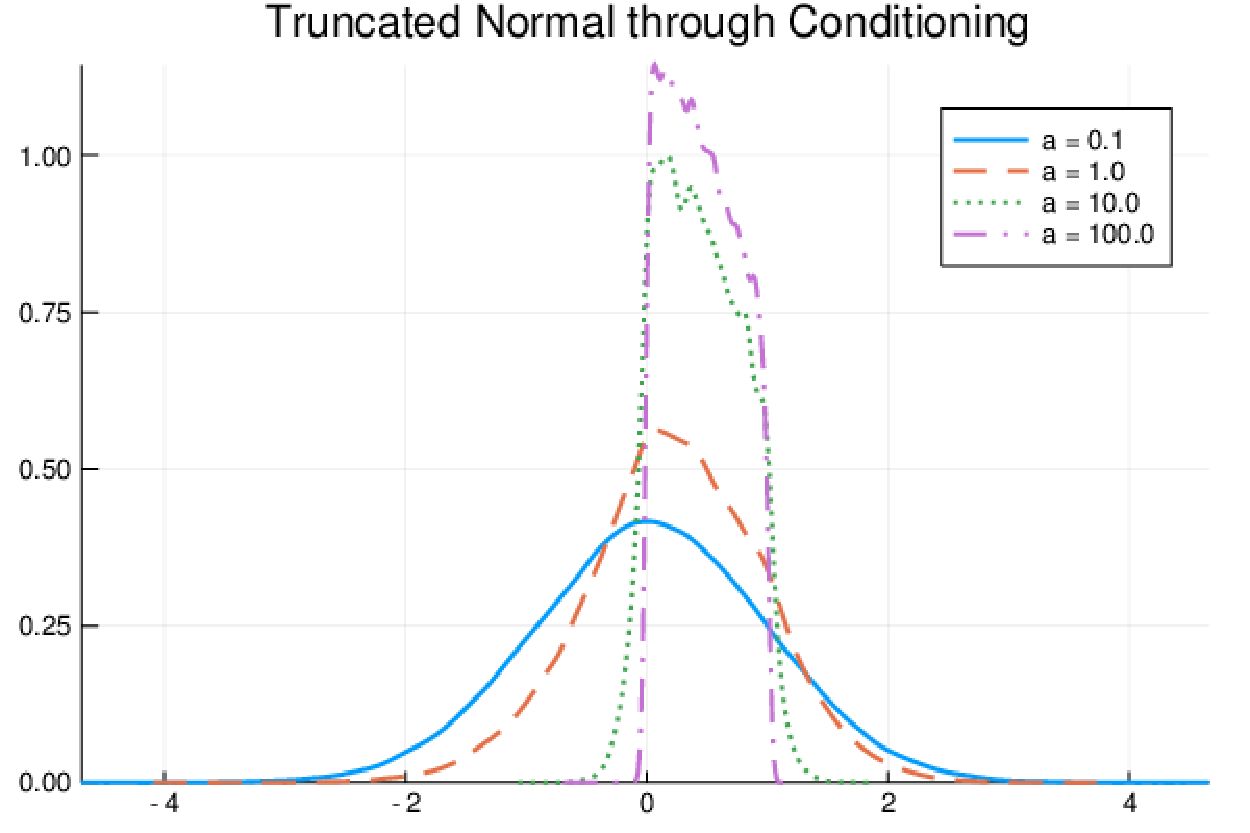
\includegraphics[width=\linewidth]{figures/truncated}
\end{minipage}%
\begin{minipage}{0.45\linewidth}
	%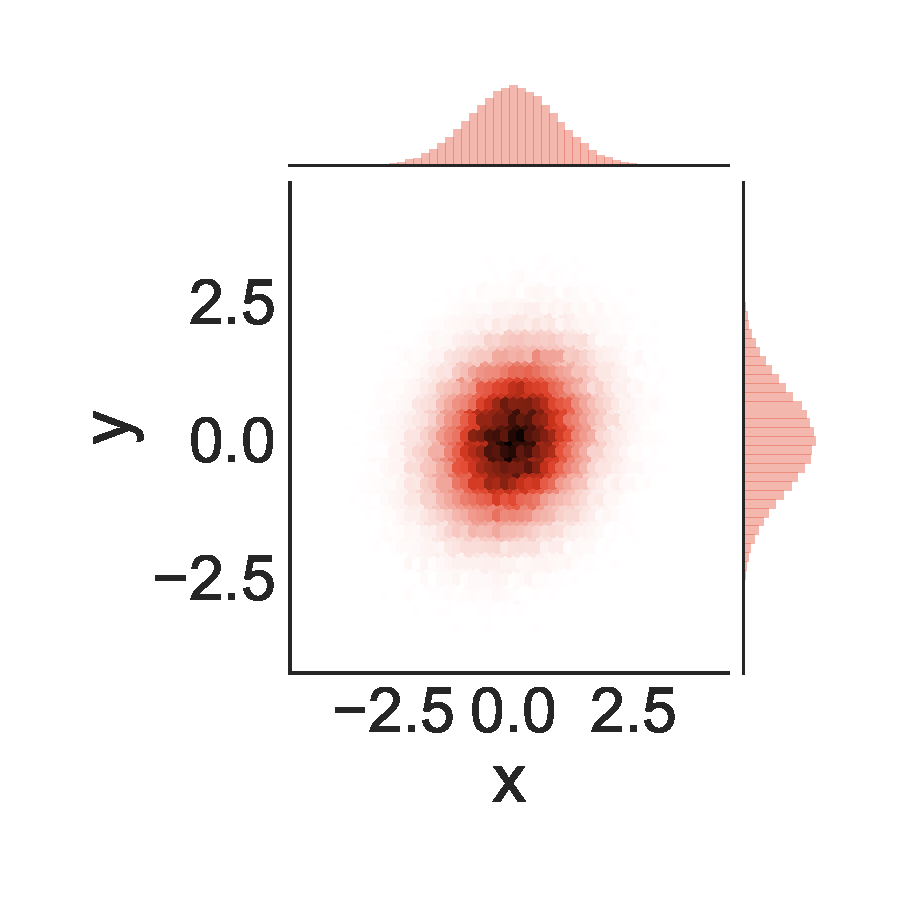
\includegraphics[width=.16\linewidth, trim={1.7cm, 1.6cm, 1.3cm, 1.5cm}, clip]{figures/0-1}
	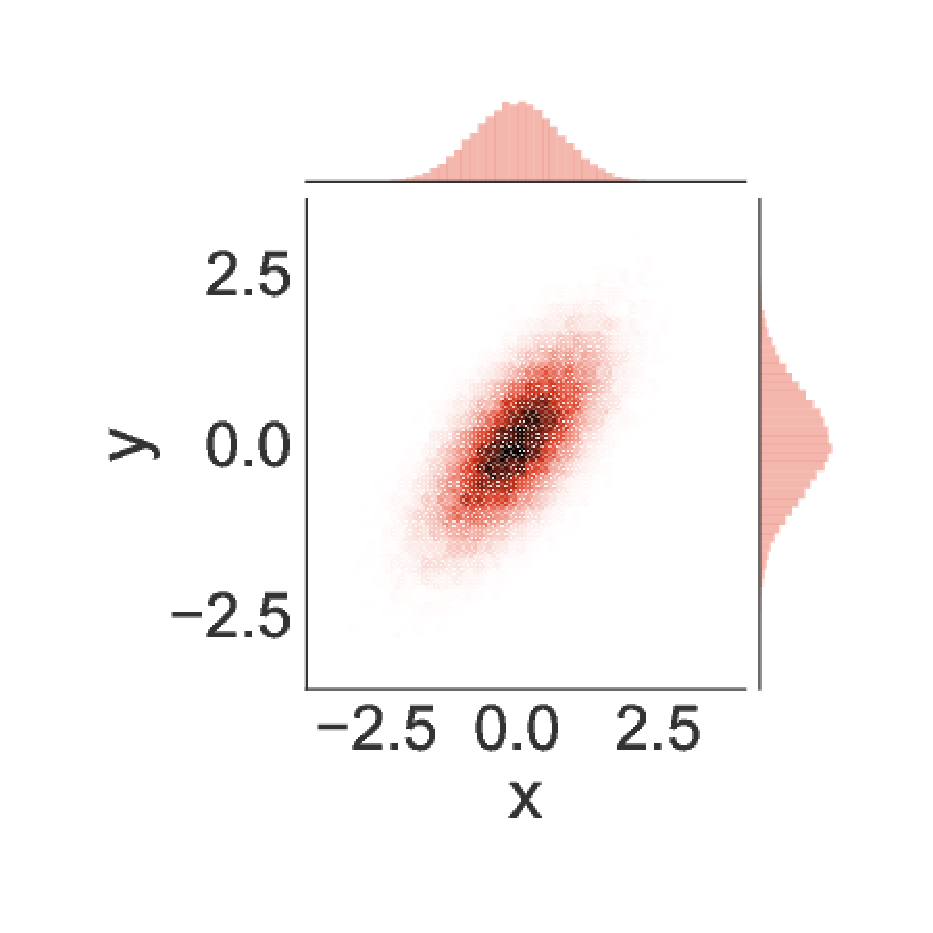
\includegraphics[width=.45\linewidth, trim={1.7cm, 1.6cm, 1.3cm, 1.5cm}, clip]{figures/1-0}
	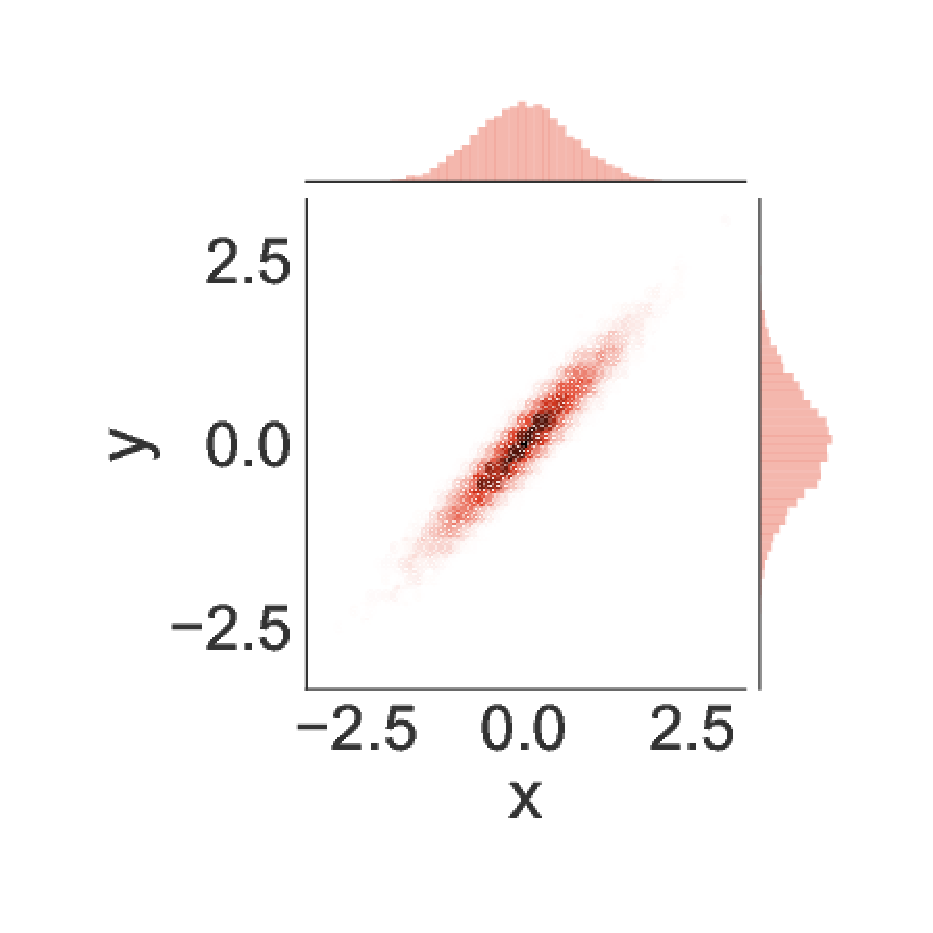
\includegraphics[width=.45\linewidth, trim={1.7cm, 1.6cm, 1.3cm, 1.5cm}, clip]{figures/10-0}
	
	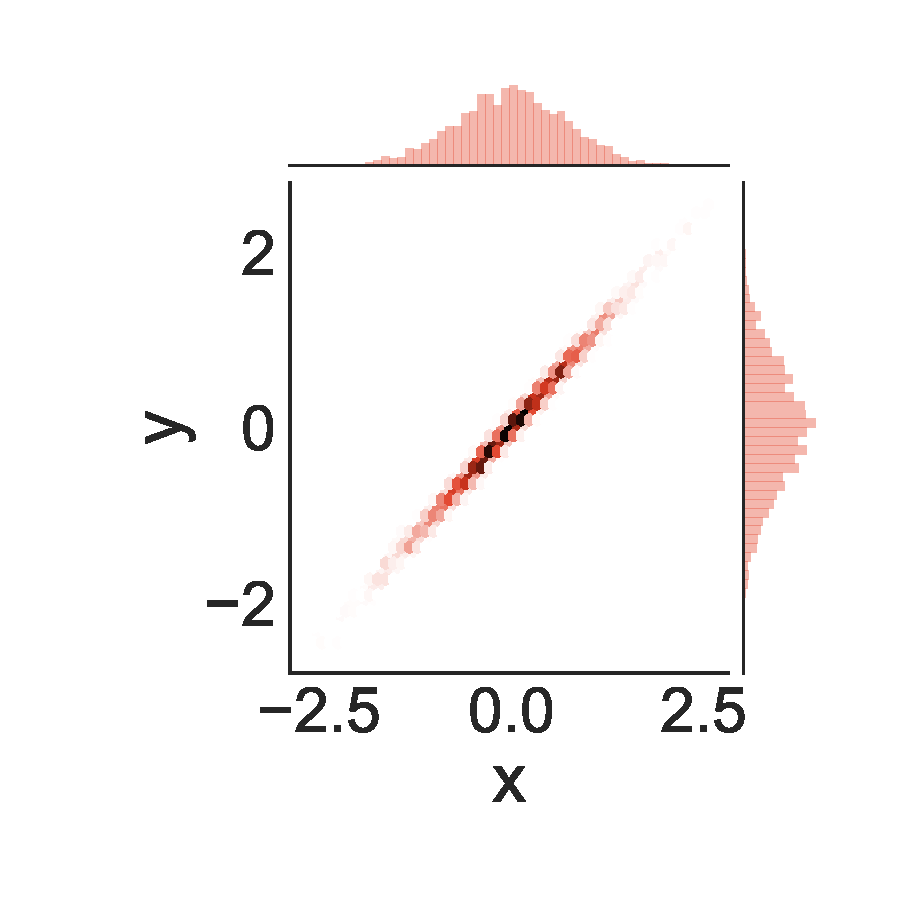
\includegraphics[width=.45\linewidth, trim={1.7cm, 1.6cm, 1.3cm, 1.5cm}, clip]{figures/100-0}
	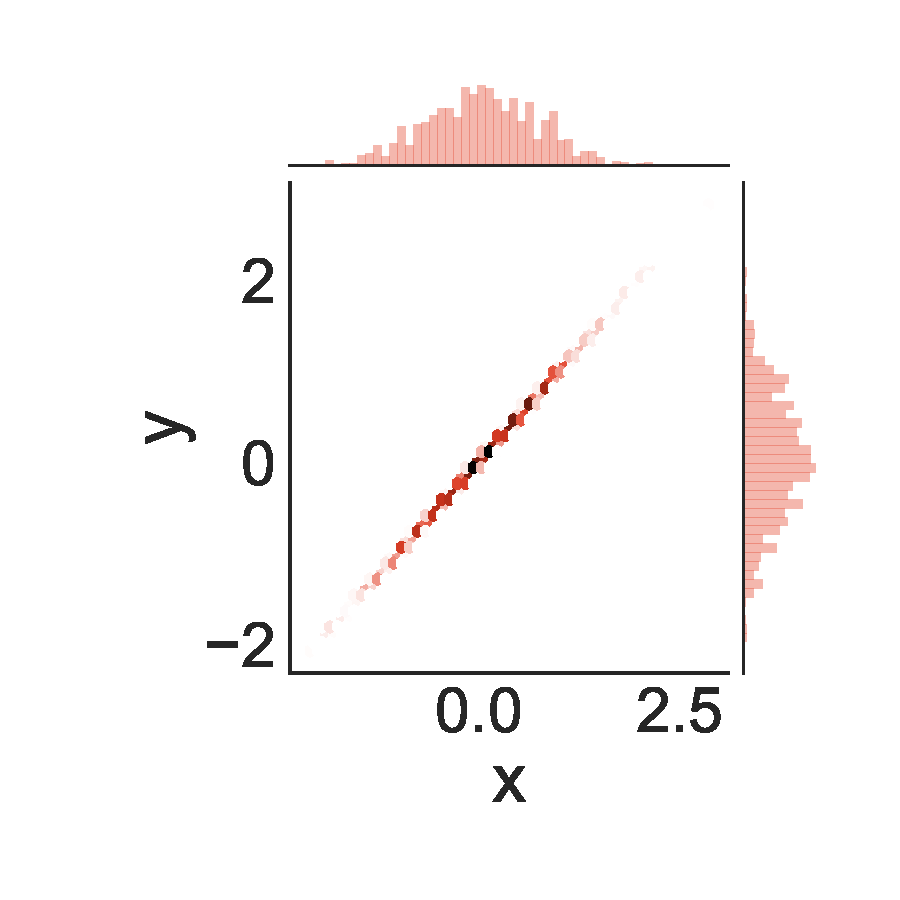
\includegraphics[width=.45\linewidth, trim={1.7cm, 1.6cm, 1.3cm, 1.5cm}, clip]{figures/1000-0}				
	
%	\fbox{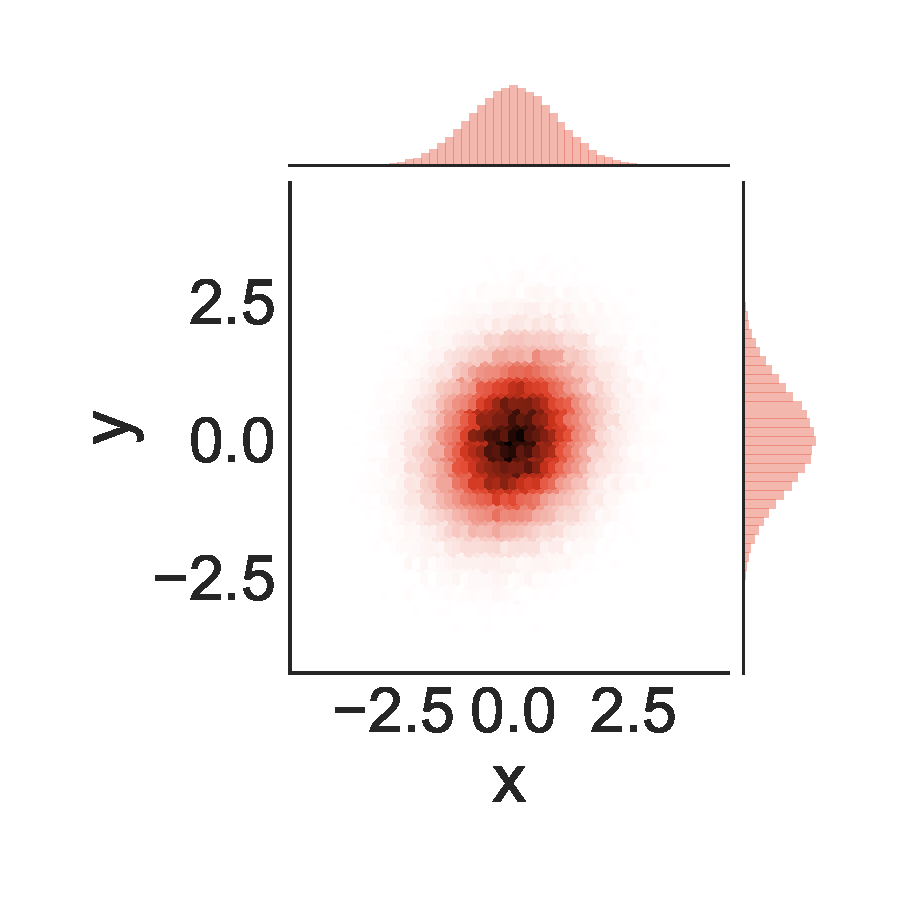
\includegraphics[width=.16\linewidth, trim={1.7cm, 1.6cm, 1.3cm, 1.5cm}, clip]{figures/0-1}}
%	\fbox{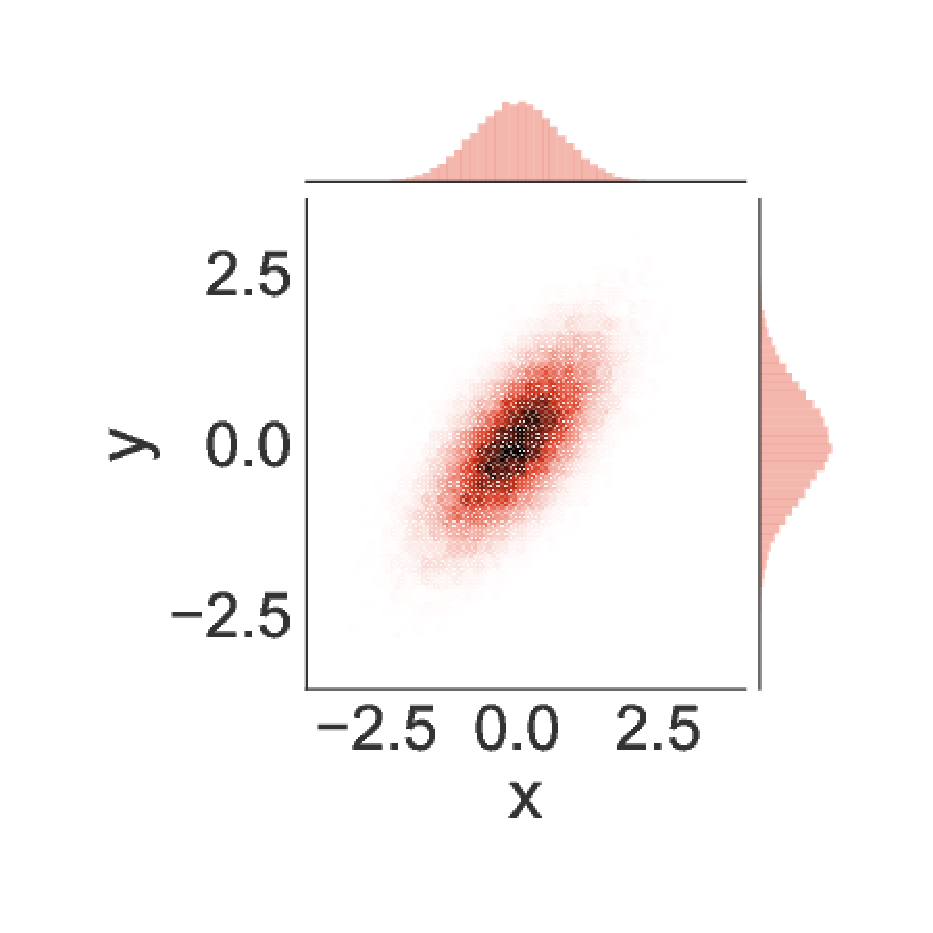
\includegraphics[width=.16\linewidth, trim={1.7cm, 1.6cm, 1.3cm, 1.5cm}, clip]{figures/1-0}}
%	\fbox{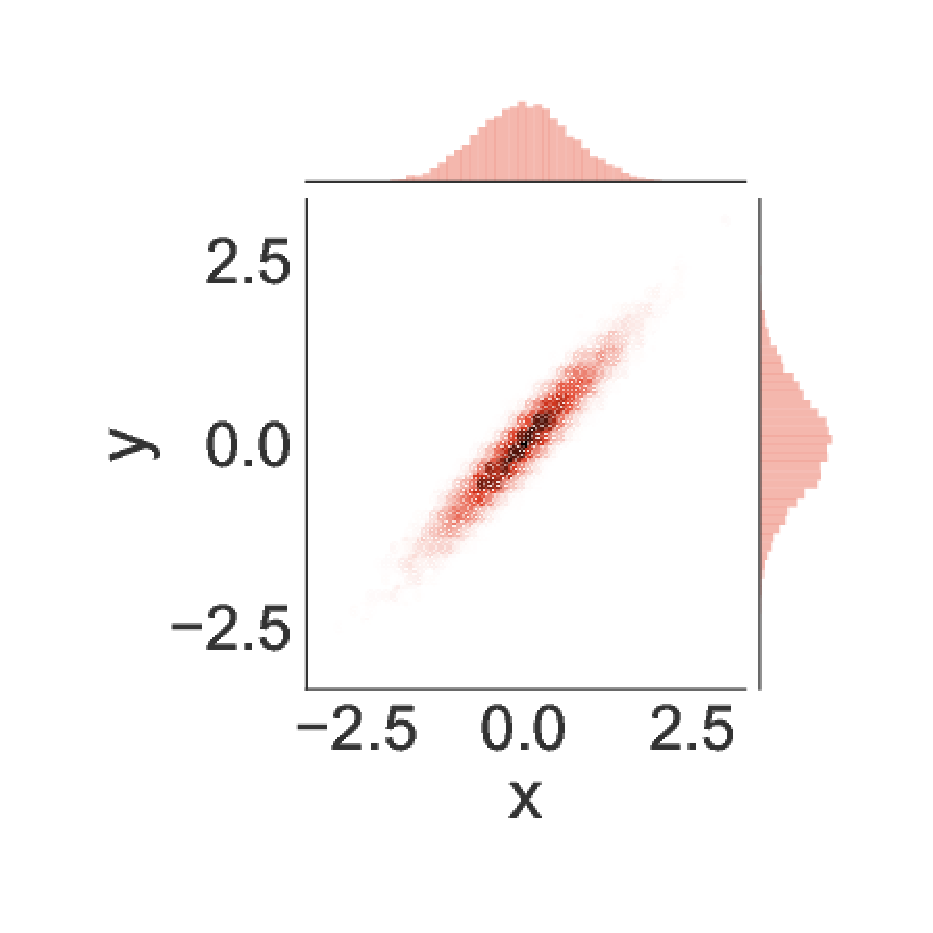
\includegraphics[width=.16\linewidth, trim={1.7cm, 1.6cm, 1.3cm, 1.5cm}, clip]{figures/10-0}}
%	\fbox{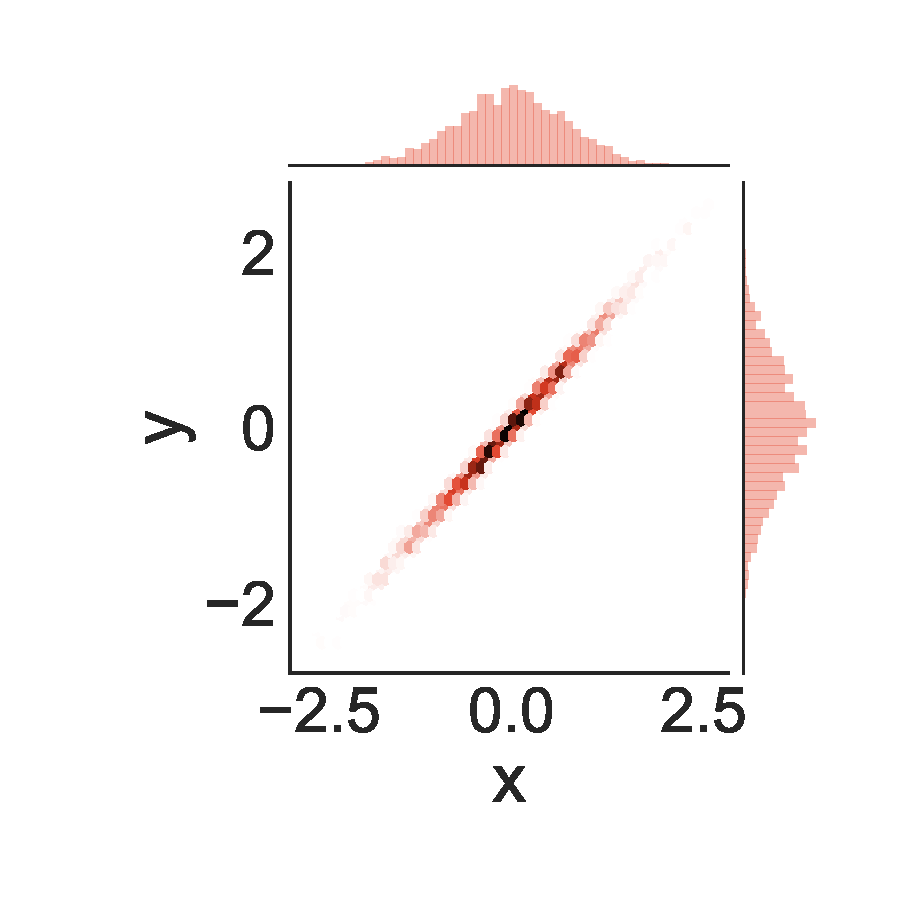
\includegraphics[width=.16\linewidth, trim={1.7cm, 1.6cm, 1.3cm, 1.5cm}, clip]{figures/100-0}}
%	\fbox{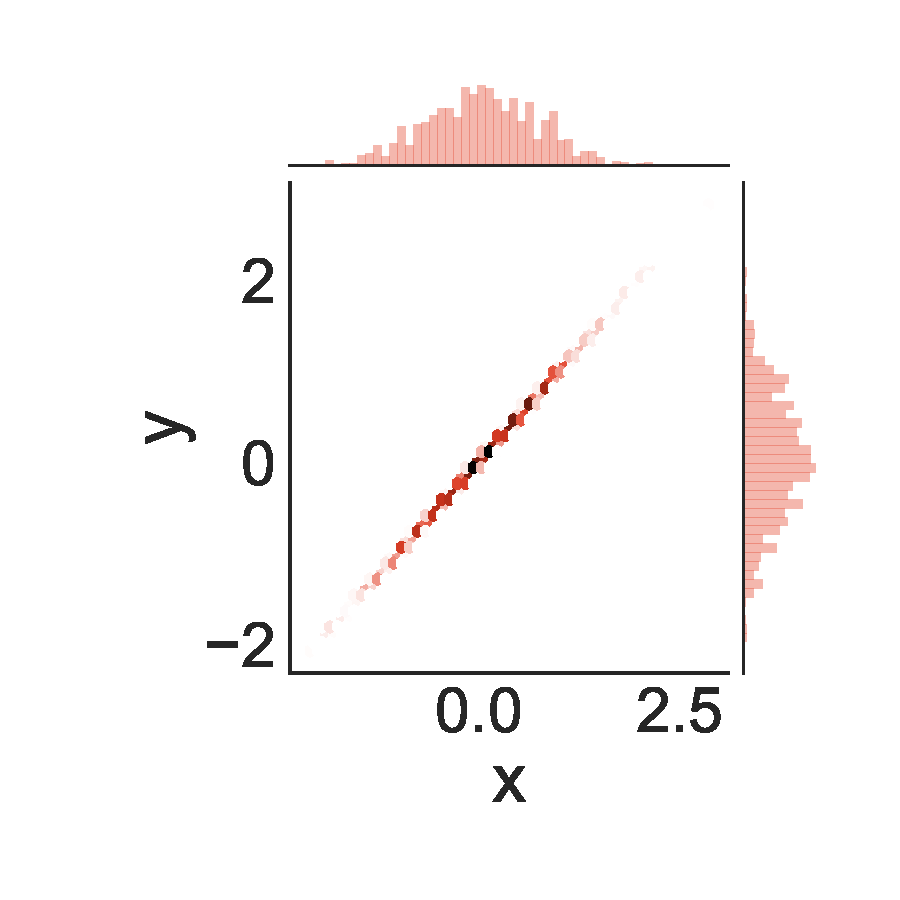
\includegraphics[width=.16\linewidth, trim={1.7cm, 1.6cm, 1.3cm, 1.5cm}, clip]{figures/1000-0}}				
	\end{minipage}
	\caption{Left: Density from samples of Gaussian truncated to $[0, 1]$ through conditioning. Right: Conditioning on $X = Y$ where $X$ and $Y$ are independent normal distributions; shown at different temperatures.}
	\label{fig:density}
\end{figure}


\paragraph{Glucose Model}
Type 2 diabetes is a prevalent and costly condition.
Keeping blood glucose within normal limits helps prevent the
long-term complications of Type 2 diabetes like diabetic neuropathy and diabetic retinopathy \citep{brownlee2006glycemic}. Models to predict the trajectories of blood glucose aid in keeping glucose within
normal limits \citep{zeevi2015personalized}. Traditional models have been built from compositions of differential equations \citep{albers2017personalized,levine2017offline} whose parameters are estimated separately for each patient. An alternative approach would be to use a flexible sequence model like an RNN. The problem with this approach is that an RNN can extrapolate to glucose values incompatible with human physiology. This is especially a problem where we have patients with only a few blood glucose measurements. To build an RNN model that respects physiology, we condition on this information using Omega. The specific Omega program is shown in the appendix.

We compare the independent RNN model to the one with declarative knowledge on a second patient from Physionet \citep{moody2001physionet}.
Figure \ref{fig:rnn-samples} plots the results performed on more than 300 pairs of patients.
We see that the conditional model simulates
more realistic glucose dynamics for the patient 
with only a short observed time-series.

% 1) Glucose modeling is a real problem \cite, \cite. 
% 2) Models have focused on ODEs \cite \cite 
% 3) Alternative is to use RNN 
% 4) RNN can produce nonsense result 
% 5) Conditioning helps


% Taken from the supplement in \cite{albers}

% \paragraph{A constrained model of glucose dynamic}
% Take glucose measurements across time $t$ from 
% N patients indexed by $i$: $x_{t,i}$.
% We model the glucose time series for each patient can be modeled independently using a recurrent neural network: 
% \begin{align*}
% W_i &\sim N(0, I) \\
% x_{t, i} &= f(x_{t-1, i}, W).
% \end{align*}
% This model treats all patients as independent. However,
% we have extra knowledge in that the average-across-time glucose levels will be similar across patients. Expressing this kind of knowledge by tying the parameters $W_i, W_j$ is a challenge because the structure of the recurrence function alters how $W$ controls the average outputs. In this sense, we would like to condition on the distance between conditional expectations being close for some distance $d$,
% \begin{align*}
% 	d_E\left(\sum_{t=1}^{T_i} E[x_{t, i} \,|\, W_i], \sum_{t=1}^{T_j} E[x_{t, j} \,|\, W_j]\right) < \delta_E,
% \end{align*}
% for all patient pairs $i, j$. Additionally, we would like to make the series smooth controlling for their variance:
% \begin{align*}
% 	d_{Var}\left(\sum_{t=1}^{T_i} Var[x_{t, i} \,|\, W_i], \sum_{t=1}^{T_j} Var[x_{t, j} \,|\, W_j]\right) < \delta_{Var},
% \end{align*}
%  We compare the independent model
% to the one with the conditional model learned on five patients. 
% We see that the conditional model simulates more realistic glucose dynamics for the patient with only a short observed time-series.

\begin{figure}[!htb]
	\centering
    %\fbox{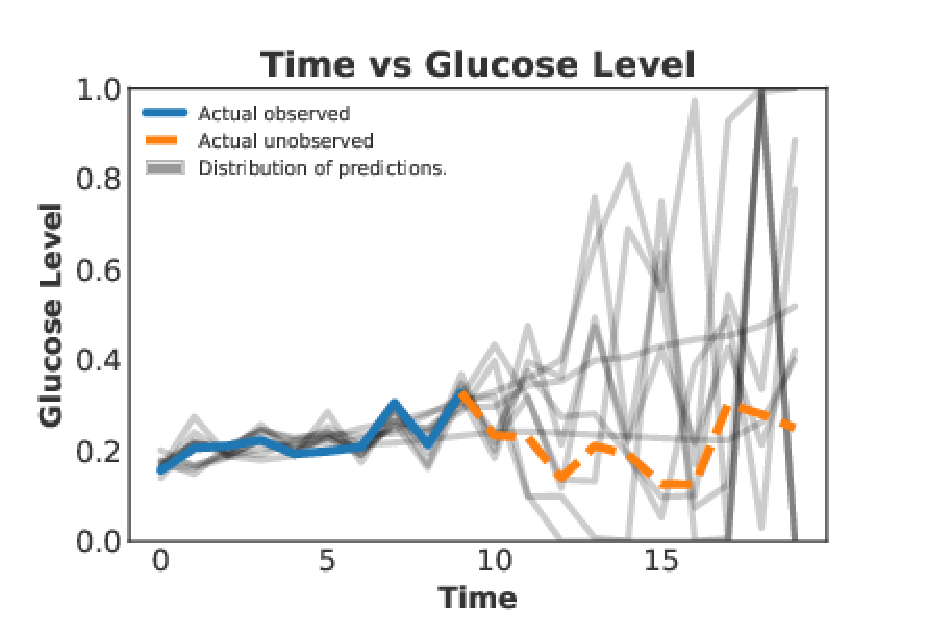
\includegraphics[width=0.30\linewidth, trim={1.cm, 0.1cm, 1.3cm, .5cm}, clip]{figures/rnnsamples-no-tie-py}}
	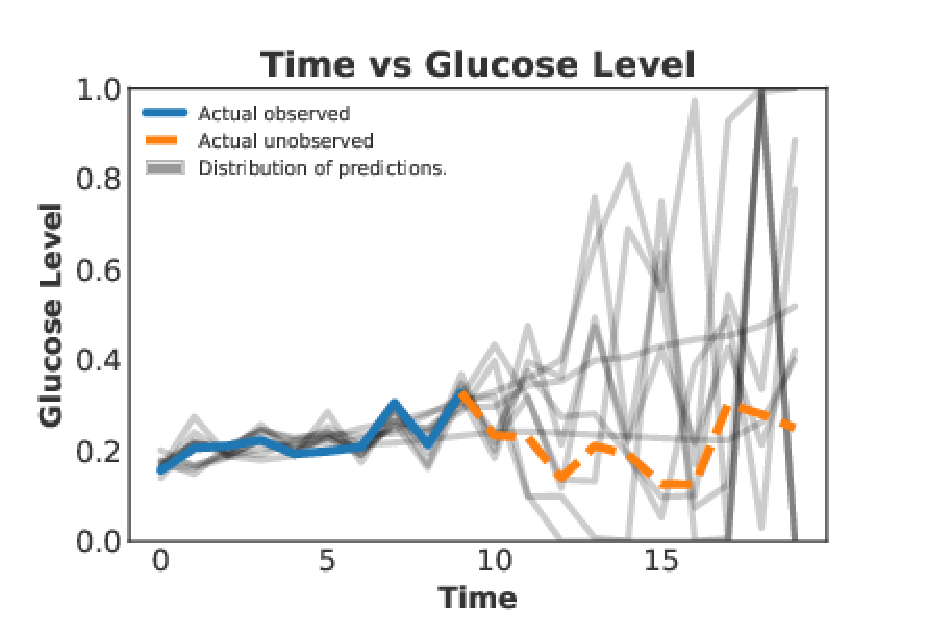
\includegraphics[width=0.30\linewidth, trim={1.cm, 0.1cm, 1.3cm, .5cm}, clip]{figures/rnnsamples-no-tie-py}
	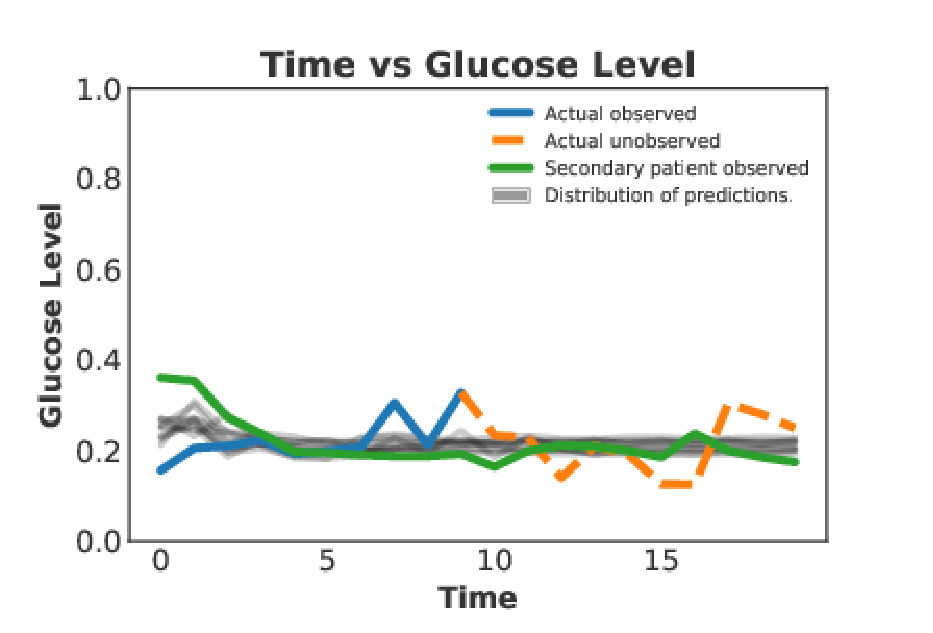
\includegraphics[width=.30\linewidth, trim={1.cm, 0.1cm, 1.3cm, .5cm}, clip]{figures/rnnsamples-py}
	%\fbox{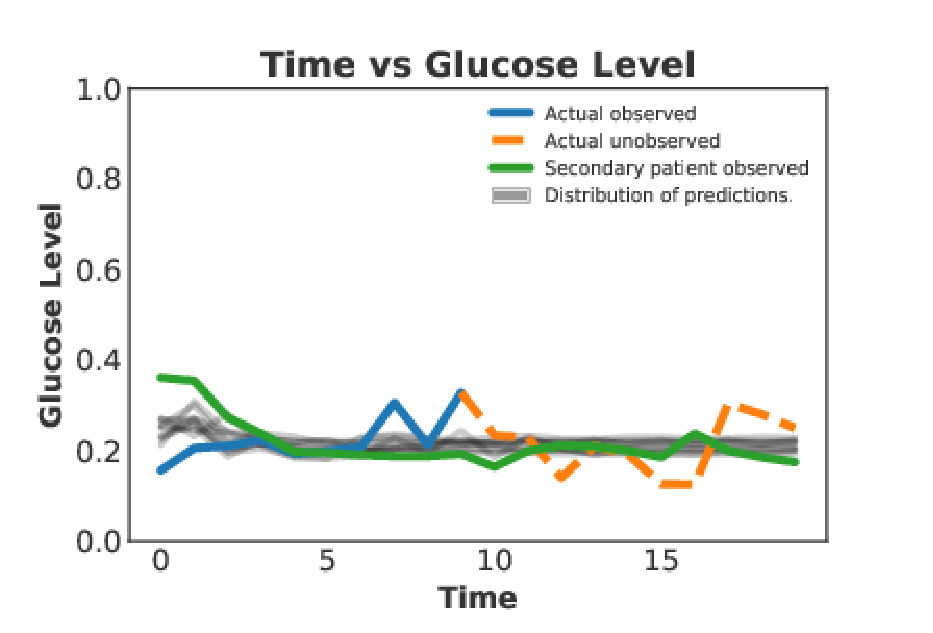
\includegraphics[width=0.30\linewidth, trim={1.cm, 0.1cm, 1.3cm, .5cm}, clip]{figures/rnnsamples-py}}
	%\fbox{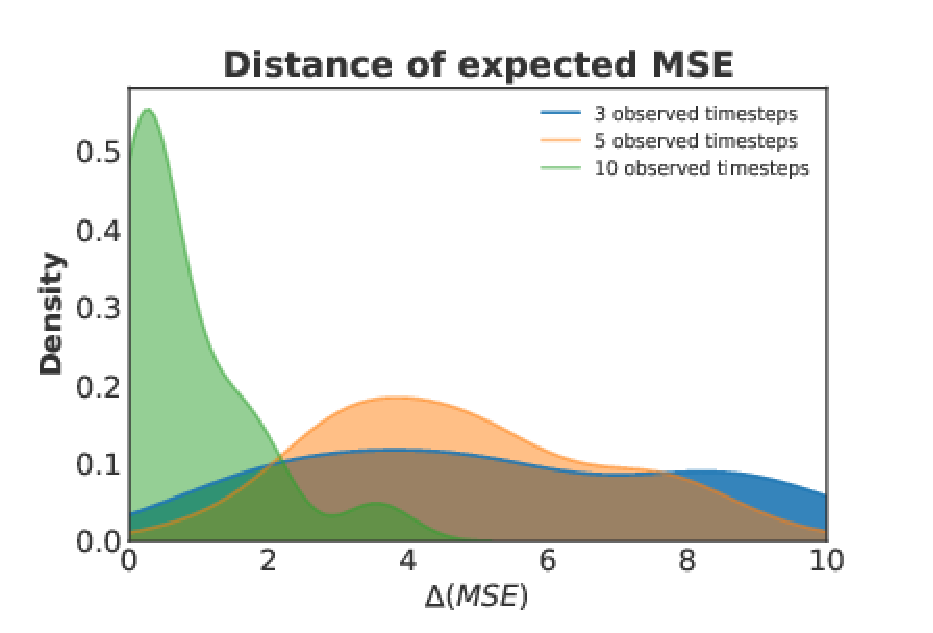
\includegraphics[width=0.30\linewidth, trim={1.cm, 0.0cm, 1.0cm, .5cm}, clip]{figures/delta_mse}}
	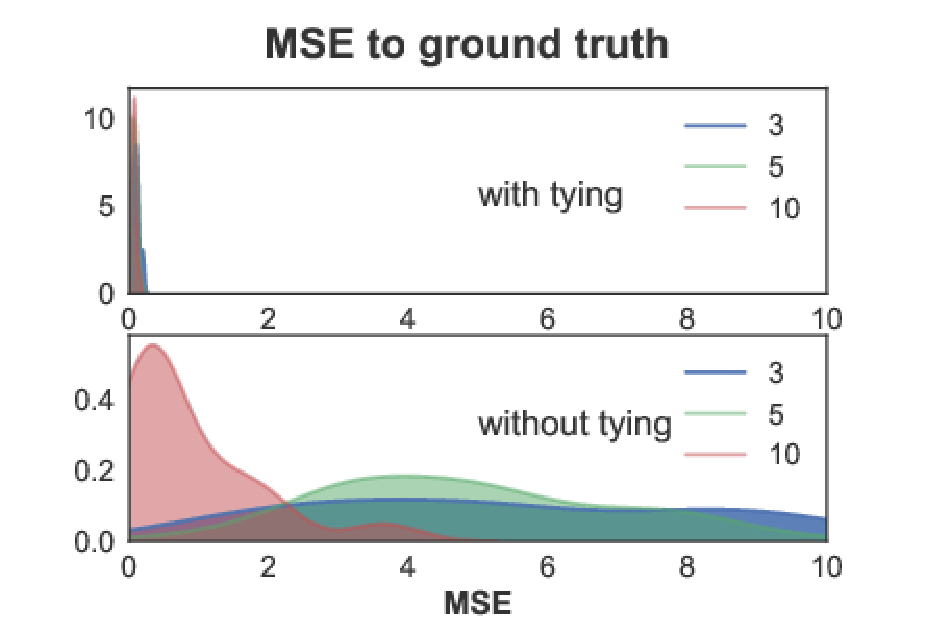
\includegraphics[width=0.30\linewidth, trim={0.7cm, 0.0cm, .7cm, .1cm}, clip]{figures/mse}
		
		\caption{Left: Actual (dotted) and predicted trajectories that were learned using a partial trajectory. Center: Distribution of predicted trajectories learned only using the first ten data points and a tie with a secondary patient. Right, top: MSE when tie is present.  Right, bottom: without tie.  Tying expectations has dramatic influence on prediction error, while as more data is observed, the effect of tying decreases.}
		\label{fig:rnn-samples}
\end{figure}



% Take the same glucose measurements from 5 patients. Make a probabilistic RNN with
% independent parameters for each patient. Then add the constraint that the means are
% close. Then look at the prediction for one patient where we remove all but the
% first few time steps and show the forward predictions are better with the added knowledge
% that the means are close across patients.


% \paragraph{Transfer Learning}
% In transfer learning, we hope to use information from one learning problem to
% help with another learning problem. One way this has been accomplished in
% deep learning is to use
% the parameters of a model learned in one domain as the initialization for the
% parameters in a another domain. We could accomplish a similar thing via conditioning
% by having the weights of both models be close. But with conditioning, this is not
% the only choice, we can have the first layer activations be close in distribution
% in both the source and target transfer domain. Concretely, consider the following
% two layer stochastic neural network for each domain where the $i$th covariate
% label pair $(x_i, y_i)$ is
% \begin{align*}
% W \sim p(W)
% z_{2, i} &\sim p(z_{2, i} | x_i, W_2) \\
% z_{1, i} &\sim p(z_{1, i} | z_{2, i}, W_1) \\
% y_{i} &\sim p(y_i | z_{1, i})
% \end{align*}


% \section{Related Work}
% \begin{itemize}

% \item Existing Notion of Probablistic Programs
% Probabilistic programming languages and the inference algorithms which support them differ primarily in how probability distributions are represented.
% % In this contribution we define the sample space as an $n$-dimensional unit hypercube
% % $\Omega = [0, 1]^n$, and by $(\omega_1,...,\omega_n)$ denote an element of $\Omega$.
% % In addition, we define $\mu$ as the Lebesgue measure.
% % Random variables are transformations of $\Omega$, and act on some or all of its dimensions.
% % For example a random variable $\mathcal{U}_{a,b}: \Omega \to \mathbb{R}$, which is distributed uniformly between $a$ and $b$ could be defined simply as:
% % $$
% % \mathcal{U}_{a,b}(\omega) = a + \omega_1(b - a)
% % $$
% \item Make explicit how the measure theortic formulation connects to the sampling process
% \end{itemize}

\section{Conclusion}
There are two ways to build models. Fix the probability space and change the definitions of random variables or change the probability space and keep random variables fixed. Both can represent a broad class of models. However the latter can 
reuse complex random variables like stochastic simulators to build new models without having to alter them.

We build new models by chaining the probability space via
conditioning. We demonstrated how conditioning on predicates can be
used to define new models that respect the knowledge given by the predicate.We developed Omega, a system that treats the underlying probability
space as a first class object. Omega relies on three primitives:
rand to create new probability spaces, functions to define new random variables, and a conditioning operator for general predicates. With these primitives, we can take a model and declare knowledge by conditioning. 

Sampling from models conditioned on arbitrary predicates poses a challenge. To address this challenge, we develop a generic scheme to soften predicates that makes them amenable to powerful MCMC algorithms like HMC. Unlike most inference algorithms, our inference algorithms operate on the abstract probability space rather than the output random variable space. 
We demonstrate Omega on many examples including models of glucose and renders.

% \section{Notation Glossary (to remove)}

% \begin{itemize}
% \item $\lift$
% \item $X$ some arbitrary random variable of type $T$
% \item $Y$ Boolean valued random variable
% \item $X_{\mid Y}$ conditional random variable of $X$ given $Y$ is true
% \item $\mean{X \mid C}$ conditional expectation of $X$ - distribution of expectations
% \end{itemize}


% \subsection*{Distributions over Random Variables}
% In some instances we want to construct to construct distributions over random variables.
% Consider the following model expressed in standard statistical notation:
% \begin{align*}
% \theta \sim \mathcal{U}(0, 1)\\
% X \sim \mathcal{N}(\theta, 1)
% \end{align*}

% $X$ is a real valued random variable.
% If instead, wish to define a distribution $\tilde{X}$ over normally distributed random variables parameterized by $\theta$ there is no standard notation.
% Treating random variables explicitly as functions, we can express the model as
% \begin{align*}
% \theta(\omega_1) &= \mathcal{U}_{0, 1}(\omega_1)\\
% X(\omega_1, \omega_2) &= \mathcal{N}_{0,1}(\omega_2) + \theta(\omega_1)
% \end{align*}

% The distribution $\tilde{X}$ over random variables can is then:
% $$
% \tilde{X}(\omega_1) =  \omega_2 \mapsto \mathcal{N}_{0,1}(\omega_2) + \theta(\omega_1)
% $$

% $\curry$ is the operator which constructs $\tilde{X}$.
% The full model is then:

% \begin{align*}
% \theta &= \mathcal{N}(0, 1)\\
% X &= \mathcal{N}(\theta, 1)\\
% \tilde{X} &= \curry(X, \theta)\\
% \tilde{X} &= \curry(\mathcal{N}(\theta, 1), \theta)
% \end{align*}

% Curry corresponds closely to the notion of \emph{currying} in functional programming.
% Let $\Omega$ be composed of several dimensions and  $X(\omega_1, \omega_2)$ be a random variable that maps from two components of $\Omega$.
% Consider a new partially applied random variable $X_{\omega_1}(\omega_2)$ that takes only one argument where the other fixed to a constant, defined as:
% $$
% X_{\omega_1}(\omega_2) = X(\omega_1, \omega_2)
% $$
% We can then define $\tilde{X}$ which constructs $X_{\omega_1}$ from $\omega_1$
% $$
% \tilde{X}(\omega_1) = \omega_1 \mapsto X_{\omega_1}
% $$
% Note that $\tilde{X}$ is a random variable.
% In programming language terminology $\tilde{X}$ is the result of currying $X$.

% $\curry(X, Y)$ curries $X$ on all the input dimensions of $Y$

\bibliography{bib}
\bibliographystyle{icml2018}

\end{document}
